\chapter{Statistics}\label{S:Statistics}

\section{Data and Statistics}\label{S:DataStats}

\begin{definition}[Data]
The function $X$ measures the outcome $\omega$ of an experiment with sample space $\Omega$ [Often, the sample space is also denoted by $S$].  Formally, $X$ is a random variable [or a random vector $X=(X_1,X_2,\ldots,X_n)$, i.e.~a vector of random variables] taking  values in the {\bf data space} $\Xz$:
\[
X(\omega):\Omega \to \Xz \ .
\]
The realisation of the RV $X$ when an experiment is performed is the observation or data $x \in \Xz$.  That is, when the experiment is performed once and it yields a specific $\omega \in \Omega$, the data $X(\omega)=x \in \Xz$ is the corresponding realisation of the RV $X$.
\end{definition}

\begin{figure}[htpb]
\caption{Sample Space, Random Variable, Realisation, Data, and Data Space.\label{F:Data}}
\vspace{2.5in}
\end{figure}

\begin{example}[Tossing a coin $n$ times]
For some given parameter $\theta \in \BB{\Theta} := [0,1]$, consider $n$ IID $\bernoulli(\theta)$ trials, i.e.~$X_1,X_2,\ldots,X_n \overset{\IID}{\sim} \bernoulli(\theta)$.  Then the random vector $X=(X_1,X_2,\ldots,X_n)$, which takes values in the data space $\Xz = \{0,1\}^n := \{ (x_1,x_2,\ldots,x_n) : x_i \in \{0,1\}, \ i=1,2,\ldots,n \}$, made up of vertices of the $n$-dimensional hyper-cube, measures the outcomes of this experiment.  A particular realisation of $X$, upon performance of this experiment, is the observation, data or data vector $(x_1,x_2,\ldots,x_n)$.  For instance, if we observed $n-1$ tails and $1$ heads, in that order, then our data vector $(x_1,x_2,\ldots,x_{n-1},x_n) = (0,0,\ldots,0,1)$.
\end{example}

\begin{figure}
\caption{Data Spaces $\Xz=\{0,1\}^2$ and $\Xz=\{0,1\}^3$ for two and three Bernoulli trials, respectively.\label{F:BernoulliDataSpace2and3}}
\centering   \makebox{\includegraphics[width=4.5in]{figures/BernoulliDataSpace2and3}}
\end{figure}

\begin{definition}[Statistic]\label{D:Statistic}
A {\bf statistic} $T$ is any 
%(measurable) 
function of the data:
\[
T(x) : \Xz \to \Tz \ .
\]
Thus, a statistic $T$ is also an RV that takes values in the space $\Tz$.  When $x \in \Xz$ is the realisation of an experiment, we let $T(x)=t$ denote the corresponding realisation of the statistic $T$. Sometimes we use $T_n(X)$ and $\Tz_n$ to emphasise that $X$ is an $n$-dimensional random vector, i.e.~$\Xz \subset \Rz^n$ 
\end{definition}

\begin{classwork}[Is data a statistic?]
Is the RV $X$, for which the realisation is the observed data $X(\omega)=x$, a statistic?  In other words, is the data a statistic? [Hint: consider the identity map $T(x)=x: \Xz \to \Tz=\Xz$.]
\end{classwork}

Next, we define two important statistics called the {\bf sample mean} and {\bf sample variance}.  Since they are obtained from the sample data, they are called {\bf sample moments}, as opposed to the {\bf population moments}.  The corresponding population moments are $\e(X_1)$ and $\V(X_1)$, respectively.
\begin{definition}[Sample Mean]\label{D:SampleMean}
From a given a sequence of RVs $X_1,X_2,\ldots,X_n$, we may obtain another RV called the $n$-samples mean or simply the sample mean:
\begin{equation}\label{E:SampleMeanRV}
T_n( \ (X_1,X_2,\ldots,X_n) \ ) = \overline{X}_n( \ (X_1,X_2,\ldots,X_n) \ ) := \frac{1}{n} \sum_{i=1}^n X_i  \ .
\end{equation}
For brevity, we write $$\overline{X}_n( \ (X_1,X_2,\ldots,X_n) \ ) \quad \text{as} \quad \overline{X}_n \ ,$$ and its realisation $$\overline{X}_n( \ (x_1,x_2,\ldots,x_n) \ ) \quad \text{as} \quad \overline{x}_n \ .$$
\end{definition}
Note that the expectation and variance of $\overline{X}_n$ are:
\begin{eqnarray}
\e(\overline{X}_n) &=& \e \left(  \frac{1}{n} \sum_{i=1}^n X_i \right) \qquad \text{{\scriptsize[by \hyperref[E:SampleMeanRV]{definition \eqref{E:SampleMeanRV}}]}} \notag \\
&=&  \frac{1}{n} \sum_{i=1}^n \e \left( X_i \right) \qquad \text{{\scriptsize [by \hyperref[E;EofLinCombofRVs]{property \eqref{E:EofLinCombofRVs}}]}} \notag
\end{eqnarray}
Furthermore, if every $X_i$ in the original sequence of RVs $X_1,X_2,\ldots$ is {\bf identically} distributed with the same expectation, by convention $\e(X_1)$, then:
\begin{equation}\label{E:ExpOfSampleMeanOfIDSeq}
\e(\overline{X}_n) 
= \frac{1}{n} \sum_{i=1}^n \e \left( X_i \right)
=  \frac{1}{n} \sum_{i=1}^n \e \left( X_1 \right) 
=  \frac{1}{n} \ n \ \e \left( X_1 \right)  = \e \left( X_1 \right) \ .
\end{equation}
Similarly, we can show that:
\begin{eqnarray}
\V(\overline{X}_n) &=& \V \left(  \frac{1}{n} \sum_{i=1}^n X_i \right) \qquad \text{{\scriptsize[by \hyperref[E:SampleMeanRV]{definition \eqref{E:SampleMeanRV}}]}} \notag \\
&=& \left( \frac{1}{n} \right)^2  \V \left( \sum_{i=1}^n X_i \right) \qquad \text{{\scriptsize [by \hyperref[E:VofAffineofRVs]{property \eqref{E:VofAffineofRVs}}]}} \notag
\end{eqnarray}
Furthermore, if the original sequence of RVs $X_1,X_2,\ldots$ is {\bf independently} distributed then:
\begin{eqnarray}
\V(\overline{X}_n) 
= \left( \frac{1}{n} \right)^2 \V \left(  \sum_{i=1}^n X_i \right) 
=  \frac{1}{n^2} \ \sum_{i=1}^n \V \left( X_i \right) \qquad \text{{\scriptsize [by \hyperref[E:VofLinCombofRVs]{property \eqref{E:VofLinCombofRVs}}]}} \notag
\end{eqnarray}
Finally, if the original sequence of RVs $X_1,X_2,\ldots$ is {\bf independently and identically} distributed with the same variance ($\V(X_1)$ by convention) then:
\begin{equation}\label{E:VarOfSampleMeanOfIIDSeq}
\V(\overline{X}_n) 
=  \frac{1}{n^2} \ \sum_{i=1}^n \V \left( X_i \right)
= \frac{1}{n^2} \ \sum_{i=1}^n \V \left( X_1 \right)
=  \frac{1}{n^2} \ n \ \V \left( X_1 \right)
=  \frac{1}{n} \ \V \left( X_1 \right) \ .
\end{equation}

\begin{labwork}[Sample mean]\label{LW:XsFromUni01Twstr101mean}
After initializing the fundamental sampler, we draw five samples and then obtain the sample mean using the {\sc Matlab} function {\tt mean}.  In the following, we will reuse the samples stored in the array {\tt XsFromUni01Twstr101}.
\begin{VrbM}
>> rand('twister',101); % initialise the fundamental Uniform(0,1) sampler 
>> XsFromUni01Twstr101=rand(1,5); % simulate n=5 IID samples from Uniform(0,1) RV
>> SampleMean=mean(XsFromUni01Twstr101);% find sample mean
>> disp(XsFromUni01Twstr101); % The data-points x_1,x_2,x_3,x_4,x_5 are:
    0.5164    0.5707    0.0285    0.1715    0.6853
>> disp(SampleMean); % The Sample mean is :
    0.3945
\end{VrbM}
We can thus use {\tt mean} to obtain the sample mean $\overline{x}_n$ of $n$ sample points $x_1,x_2,\ldots,x_n$.

We may also obtain the sample mean using the {\tt sum} function and a division by sample size:
\begin{VrbM}
>> sum(XsFromUni01Twstr101) % take the sum of the elements of the XsFromUni01Twstr101 array
ans =    1.9723
>> sum(XsFromUni01Twstr101) / 5 % divide the sum by the sample size 5
ans =    0.3945
\end{VrbM}

We can also obtain the sample mean via matrix product or multiplication as follows:
\begin{VrbM}
>> size(XsFromUni01Twstr101) % size(SomeArray) gives the size or dimensions of the arrar SomeArray
ans =     1     5
>> ones(5,1) % here ones(5,1) is an array of 1's with size or dimension 5 X 1
ans =
     1
     1
     1
     1
     1
>> XsFromUni01Twstr101 * ones(5,1) % multiplying an 1 X 5 matrix with a 5 X 1 matrix of Ones
ans =    1.9723
>> XsFromUni01Twstr101 * ( ones(5,1) * 1/5) % multiplying an 1 X 5 matrix with a 5 X 1 matrix of 1/5 's
ans =    0.3945
\end{VrbM}
\end{labwork}

\begin{definition}[Sample Variance \& Standard Deviation]
From a given a sequence of random variables $X_1,X_2,\ldots,X_n$, we may obtain another statistic called the $n$-samples variance or simply the sample variance :
\begin{equation}\label{E:SampleVarianceRV}
T_n( \ (X_1,X_2,\ldots,X_n) \ ) = S^2_n( \ (X_1,X_2,\ldots,X_n) \ )  := \frac{1}{n-1} \sum_{i=1}^n {(X_i - \overline{X}_n)^2}  \ .
\end{equation}
For brevity, we write $S^2_n( \ (X_1,X_2,\ldots,X_n) \ )$ as $S^2_n$ and its  realisation $S^2_n( \ (x_1,x_2,\ldots,x_n) \ )$ as $s^2_n$.

Sample standard deviation is simply the square root of sample variance:
\begin{equation}\label{E:SampleStdDevRV}
S_n( \ (X_1,X_2,\ldots,X_n) \ ) = \sqrt{S^2_n( \ (X_1,X_2,\ldots,X_n) \ )}
\end{equation}
For brevity, we write $S_n( \ (X_1,X_2,\ldots,X_n) \ )$ as $S_n$ and its  realisation $S_n( \ (x_1,x_2,\ldots,x_n) \ )$ as $s_n$.
\end{definition}
Once again, if $X_1,X_2,\ldots,X_n \overset{\IID}{\sim} X_1$, the expectation of the sample variance is:
\[
\e(S^2_n) = \V(X_1) \ .
\]
\begin{labwork}[Sample variance and sample standard deviation]\label{LW:XsFromUni01Twstr101varstd}
We can compute the sample variance and sample standard deviation for the five samples stored in the array {\tt XsFromUni01Twstr101} from \hyperref[LW:XsFromUni01Twstr101mean]{Labwork \ref*{LW:XsFromUni01Twstr101mean}} using {\sc Matlab}'s functions {\tt var} and {\tt std}, respectively.
\begin{VrbM}
>> disp(XsFromUni01Twstr101); % The data-points x_1,x_2,x_3,x_4,x_5 are :
    0.5164    0.5707    0.0285    0.1715    0.6853
>> SampleVar=var(XsFromUni01Twstr101);% find sample variance
>> SampleStd=std(XsFromUni01Twstr101);% find sample standard deviation
>> disp(SampleVar) % The sample variance is:
    0.0785
>> disp(SampleStd) % The sample standard deviation is:
    0.2802
\end{VrbM}
\end{labwork}
It is important to bear in mind that the statistics such as sample mean and sample variance are random variables and have an underlying distribution.

\begin{definition}[Order Statistics]
Suppose $X_1,X_2,\ldots,X_n \overset{\IID}{\sim} F$, where $F$ is the DF from the set of all DFs over the real line.  Then, the $n$-sample {\bf order statistics} $X_{([n])}$ is:
\begin{equation}\label{E:OrderStatistics}
X_{([n])}( \ (X_1,X_2,\ldots,X_n) \ ) := \left(  X_{(1)},X_{(2)}, \ldots X_{(n)} \right), \text{ such that, }
 X_{(1)} \leq X_{(2)} \leq \ldots \leq X_{(n)}  \ .
\end{equation}
For brevity, we write $X_{([n])}( \ (X_1,X_2,\ldots,X_n) \ )$ as $X_{([n])}$ and its realisation $X_{([n])}( \ (x_1,x_2,\ldots,x_n) \ )$ as $x_{([n])} = (  x_{(1)},x_{(2)}, \ldots x_{(n)} )$.
\end{definition}
Without going into the details of how to sort the data in ascending order to obtain the order statistics (an elementary topic of an Introductory Computer Science course), we simply use {\sc Matlab}'s function {\tt sort} to obtain the order statistics, as illustrated in the following example.
\begin{labwork}[Order statistics and sorting]\label{LW:SortedXsFromUni01Twstr101}
The order statistics for the five samples stored in {\tt XsFromUni01Twstr101} from \hyperref[LW:XsFromUni01Twstr101mean]{Labwork \ref*{LW:XsFromUni01Twstr101mean}} can be computed using {\tt sort} as follows:
\begin{VrbM}
>> disp(XsFromUni01Twstr101); % display the sample points
    0.5164    0.5707    0.0285    0.1715    0.6853
>> SortedXsFromUni01Twstr101=sort(XsFromUni01Twstr101); % sort data
>> disp(SortedXsFromUni01Twstr101); % display the order statistics
    0.0285    0.1715    0.5164    0.5707    0.6853
\end{VrbM}
Therefore, we can use {\tt sort} to obtain our order statistics $x_{(1)},x_{(2)},\ldots,x_{(n)}$ from $n$ sample points $x_1,x_2,\ldots,x_n$.
\end{labwork}

Next, we will introduce a family of common statistics, called the $q^{\text{th}}$ quantile, by first defining the function:
\begin{definition}[Inverse DF or Inverse CDF or Quantile Function]
Let $X$ be an RV with DF $F$.  The {\bf inverse DF} or {\bf inverse CDF} or {\bf quantile function} is:
\begin{equation}\label{E:InverseCDF}
F^{[-1]}(q) := \inf { \{ x: F(x) > q \}}, \quad \text{ for some $q \in [0,1]$} \ .
\end{equation} 
If $F$ is strictly increasing and continuous then $F^{[-1]}(q)$ is the unique $x \in \Rz$ such that $F(x)=q$.
\end{definition}
A {\bf functional} is merely a function of another function.  Thus, $T(F): \{ \text{All DFs }\} \to \Tz$, being a map or function from the space of DFs to its range $\Tz$, is a functional.  Some specific examples of functionals we have already seen include:
\begin{enumerate}
\item The {\bf mean} of RV $X \sim F$ is a function of the DF $F$:  
\[
T(F) = \e(X) = \int x\,dF(x) \ .
\]
\item The {\bf variance} of RV $X \sim F$ is a function of the DF $F$:  
\[
T(F) = \e(X-\e(X))^2 = \int (x-\e(X))^2\,dF(x) \ .
\]
\item The {\bf value of DF at a given $x \in \Rz$} of RV $X \sim F$ is also a function of DF $F$:
\[
T(F) = F(x) \  .
\]
\end{enumerate}
Other functionals of $F$ that depend on the quantile function $F^{[-1]}$ are:
\begin{enumerate}
\item The {\bf $q^{\text{th}}$ quantile} of RV $X \sim F$: 
\[
T(F) = F^{[-1]}(q) \ \text{ where } q \in [0,1] \ .
\]
\item The {\bf first quartile} or the {\bf $0.25^{\text{th}}$ quantile} of the RV $X \sim F$: 
\[
T(F) = F^{[-1]}(0.25) \ .
\]
\item The {\bf median} or the {\bf second quartile} or the {\bf $0.50^{\text{th}}$ quantile} of the RV $X \sim F$: 
\[
T(F) = F^{[-1]}(0.50) \  .
\]
\item The {\bf third quartile} or the {\bf $0.75^{\text{th}}$ quantile} of the RV $X \sim F$: 
\[
T(F) = F^{[-1]}(0.75) \ .
\]
\end{enumerate}

\begin{definition}[Empirical Distribution Function (EDF or ECDF)]\label{D:ECDF}
Suppose we have $n$ IID RVs, $X_1,X_2,\ldots,X_n \overset{\IID}{\sim} F$, where $F$ is a DF from the set of all DFs over the real line.  Then, the $n$-sample empirical distribution function (EDF or ECDF) is the discrete  distribution function $\widehat{F}_n$ that puts a probability mass of $1/n$ at each sample or data point $x_i$:
\begin{eqnarray} \label{E:ECDF}
\widehat{F}_n(x) = \frac{ \sum_{i=1}^n \BB{1}(X_i \leq x) }{n} \ ,  & \quad where \qquad
\BB{1}(X_i \leq x) :=
\begin{cases}
& 1  \quad \text{if $x_i \leq x$} \\
& 0  \quad \text{if $x_i > x$} 
\end{cases}
\end{eqnarray}
\end{definition}

\begin{labwork}[Plot of empirical CDF]\label{LW:ECDF}
Let us plot the ECDF for the five samples drawn from the $Uniform(0,1)$ RV in \hyperref[LW:XsFromUni01Twstr101mean]{Labwork \ref*{LW:XsFromUni01Twstr101mean}} using the {\sc Matlab} function {\tt ECDF} (given in \hyperref[Mf:ECDF]{Labwork \ref*{Mf:ECDF}}).  Let us super-impose the samples and the true DF as depicted in \hyperref[F:plotUniform01ECDF5]{Figure \ref*{F:plotUniform01ECDF5}} with the following script:
{\VrbMf[label=plotunifecdf.m]{scripts/plotunifecdf.m}}

\begin{figure}[htpb]
\caption{Plot of the DF of $\uniform(0,1)$, five IID samples from it, and the ECDF $\widehat{F}_5$ for these five data points $x=(x_1,x_2,x_3,x_4,x_5)=(0.5164,    0.5707,    0.0285,    0.1715,    0.6853)$ that jumps by $1/5=0.20$ at each of the five samples.\label{F:plotUniform01ECDF5}}
\centering   \makebox{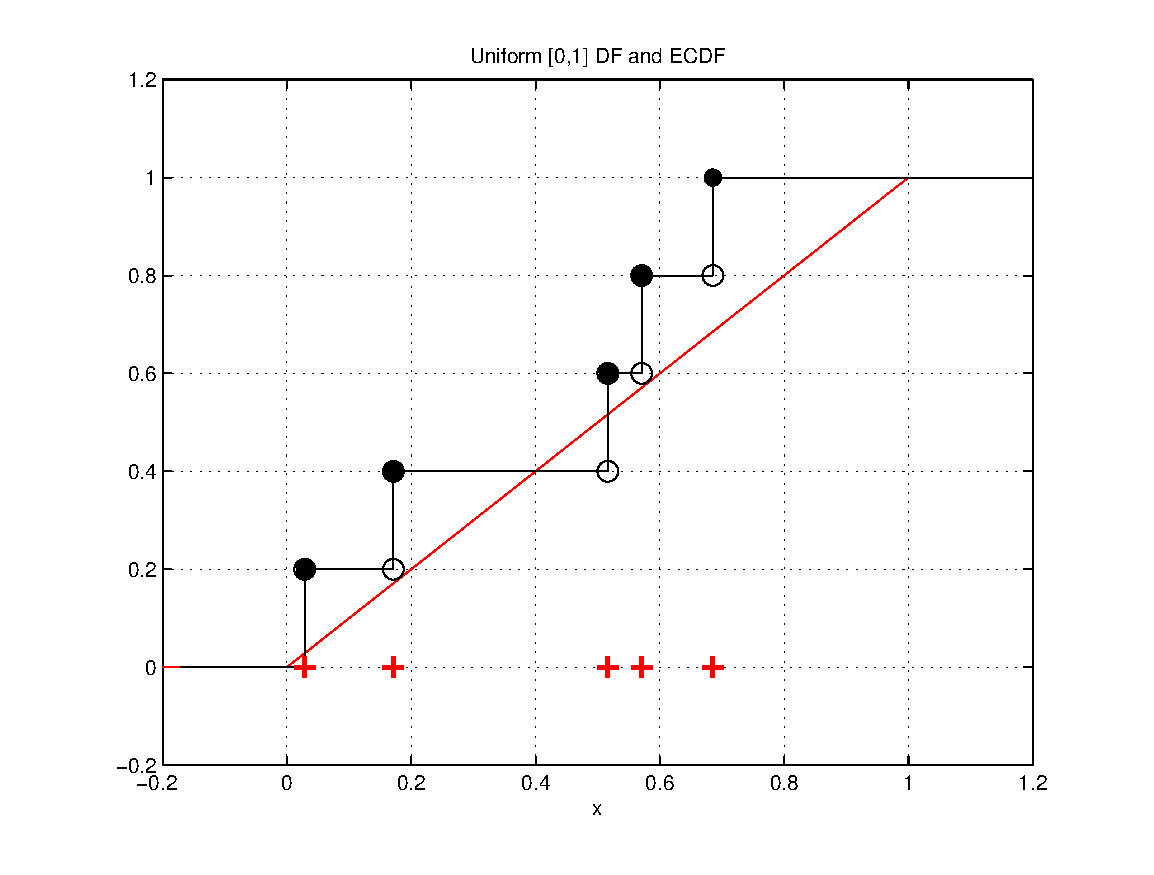
\includegraphics[width=4.5in]{figures/plotUniform01ECDF5}}
\end{figure}
\end{labwork}

\begin{definition}[$q^{\text{th}}$ Sample Quantile]
For some $q \in [0,1]$ and $n$ IID RVs $X_1,X_2,\ldots,X_n \overset{\IID}{\sim} F$, we can obtain the ECDF $\widehat{F}_n$ using \eqref{E:ECDF}.  The {\bf $q^{\text{th}}$ sample quantile} is defined as the statistic (statistical functional):
\begin{equation}\label{E:qthSampleQuantile}
T(\widehat{F}_n) = \widehat{F}_n^{[-1]}(q) := \inf{ \{ x:  \widehat{F}_n^{[-1]}(x) \geq q \} } \ .
\end{equation}
By replacing $q$ in this definition of the $q^{\text{th}}$ sample quantile by $0.25$, $0.5$ or $0.75$, we obtain the first, second ({\bf sample median}) or third {\bf sample quartile}, respectively.
\end{definition}

The following algorithm can be used to obtain the $q^{\text{th}}$ sample quantile of $n$ IID samples $(x_1,x_2,\ldots,x_n)$ on the basis of their order statistics $(x_{(1)},x_{(2)},\ldots,x_{(n)})$.
\begin{algorithm}
\caption{$q^{\text{th}}$ Sample Quantile of Order Statistics}
\label{A:qthSampleQuantile}
\begin{algorithmic}[1]
\STATE {
{\it input:} 
\begin{enumerate}
\item $q$ in the $q^{\text{th}}$ sample quantile, i.e.~the argument $q$ of $ \widehat{F}_n^{[-1]}(q)$,
\item order statistic $(x_{(1)},x_{(2)},\ldots,x_{(n)})$, i.e.~the sorted $(x_1,x_2,\ldots,x_n)$, where $n>0$.
\end{enumerate}
}
\STATE {\it output:} $ \widehat{F}_n^{[-1]}(q)$, the $q^{\text{th}}$ sample quantile
\STATE $i \gets \lfloor (n-1) q \rfloor$
\STATE $\delta \gets (n-1) q - i$
\IF {$i = n-1$}
\STATE {$ \widehat{F}_n^{[-1]}(q) \gets x_{(i+1)}$}
\ELSE
\STATE $ \widehat{F}_n^{[-1]}(q) \gets (1 - \delta) x_{(i+1)} + \delta x_{(i+2)}$
\ENDIF
\STATE {{\it return:} $ \widehat{F}_n^{[-1]}(q)$}
\end{algorithmic}
\end{algorithm}

The $q^{\text{th}}$ sample quantile, $ \widehat{F}_n^{[-1]}(q)$, is found by interpolation from the order statistics $(x_{(1)},x_{(2)},\ldots,x_{(n)})$ of the $n$ data points $(x_1,x_2,\ldots,x_n)$, using the formula:
\[
 \widehat{F}_n^{[-1]}(q) = (1 - \delta) x_{(i+1)} + \delta x_{(i+2)}, \quad \text{where, }
\quad i = \lfloor (n-1) q \rfloor  \quad \text{ and }
\quad \delta = (n-1) q -  \lfloor (n-1) q \rfloor \ .
\]
Thus, the {\bf sample minimum} of the data points $(x_1,x_2,\ldots,x_n)$ is given by $ \widehat{F}_n^{[-1]}(0)$, the {\bf sample maximum} is given by $ \widehat{F}_n^{[-1]}(1)$ and the {\bf sample median} is given by $ \widehat{F}_n^{[-1]}(0.5)$, etc.
\begin{labwork}[The $q^{\text{th}}$ sample quantile]\label{LW:qthSampleQuantile}
Use the implementation of \hyperref[A:qthSampleQuantile]{Algorithm \ref*{A:qthSampleQuantile}} in \hyperref[Mf:qthSampleQuantile]{Labwork \ref*{Mf:qthSampleQuantile}} as the {\sc Matlab} function {\tt qthSampleQuantile} to find the $q^{\text{th}}$ sample quantile of two simulated data arrays:
\begin{enumerate}
\item {\tt SortedXsFromUni01Twstr101}, the order statistics that was constructed in \hyperref[LW:SortedXsFromUni01Twstr101]{Labwork \ref*{LW:SortedXsFromUni01Twstr101}} and
\item Another sorted array of $7$ samples called {\tt SortedXs}
\end{enumerate}
\begin{VrbM}
>> disp(SortedXsFromUni01Twstr101)
    0.0285    0.1715    0.5164    0.5707    0.6853
>> rand('twister',420);
>> SortedXs=sort(rand(1,7));
>> disp(SortedXs)
    0.1089    0.2670    0.3156    0.3525    0.4530    0.6297    0.8682
>> for q=[0, 0.25, 0.5, 0.75, 1.0]
       disp([q, qthSampleQuantile(q,SortedXsFromUni01Twstr101) ...
                qthSampleQuantile(q,SortedXs)])
   end
         0    0.0285    0.1089
    0.2500    0.1715    0.2913
    0.5000    0.5164    0.3525
    0.7500    0.5707    0.5414
    1.0000    0.6853    0.8682
\end{VrbM}
\end{labwork}

\section{Exploring Data and Statistics}\label{S:ExploringData}

\subsection{Univariate Data}
A {\bf histogram} is a graphical representation of the frequency with which elements of a data array:
$$x = (x_1,x_2,\ldots,x_n) \ ,$$ 
of real numbers fall within each of the $m$ intervals or {\bf bins} of some {\bf interval partition}:
$$b := ( b_1, b_2, \ldots, b_m ) := ( [\underline{b}_1,\overline{b}_1], [\underline{b}_2,\overline{b}_2], \ldots, [\underline{b}_m,\overline{b}_m] )$$
of the {\bf data range} of $x$ given by the closed interval: 
$$\C{R}(x) := [\min \{x_1,x_2,\ldots,x_n \}, \max \{x_1,x_2,\ldots,x_n \}] \ .$$  
Elements of this partition $b$ are called bins, their mid-points are called {\bf bin centres}:
$$c := ( c_1, c_2, \ldots, c_m ) := ( (\underline{b}_1+\overline{b}_1)/2, (\underline{b}_2 + \overline{b}_2)/2, \ldots, (\underline{b}_m + \overline{b}_m)/2 )$$
and their overlapping boundaries, i.e.~$\overline{b}_i=\underline{b}_{i+1}$ for $1 \leq i < m$, are called {\bf bin edges}:
$$d := (d_1,d_2,\ldots,d_{m+1}) := (\underline{b}_1, \underline{b}_2, \ldots, \underline{b}_{m-1}, \underline{b}_m, \overline{b}_m) \ .$$ 
For a given partition of the data range $\C{R}(x)$ or some superset of $\C{R}(x)$, three types of histograms are possible: frequency histogram, relative frequency histogram and density histogram.  Typically, the partition $b$ is assumed to be composed of $m$ overlapping intervals of the same width $w=\overline{b}_i - \underline{b}_i$ for all $i=1,2,\ldots,m$.  Thus, a histogram can be obtained by a set of bins along with their corresponding {\bf heights}:
$$h = (h_1,h_2,\ldots,h_m) \ , \text{ where } h_k := g(\# \{x_i : x_i \in b_k\} )$$
Thus, $h_k$, the height of the $k$-th bin, is some function $g$ of the number of data points that fall in the bin $b_k$ Formally, a histogram is a sequence of ordered pairs:
$$\left(  (b_1,h_1), (b_2,h_2), \ldots, (b_m,h_m) \right) \ .$$

Given a partition $b$, a {\bf frequency histogram} is the histogram:
$$\left(  (b_1,h_1), (b_2,h_2), \ldots, (b_m,h_m) \right) \ , \text{ where } h_k := \# \{x_i : x_i \in b_k\} \ ,$$
a {\bf relative frequency histogram} is the histogram:
$$\left(  (b_1,h_1), (b_2,h_2), \ldots, (b_m,h_m) \right) \ , \text{ where } h_k := n^{-1} \# \{x_i : x_i \in b_k\} \ ,$$
and a {\bf density histogram} is the histogram:
$$\left(  (b_1,h_1), (b_2,h_2), \ldots, (b_m,h_m) \right) \ , \text{ where } h_k := (w_k n)^{-1} \# \{x_i : x_i \in b_k\} \ , w_k := \overline{b}_k - \underline{b}_k \ .$$
  
\begin{figure}[htpb]
\caption{Frequency, Relative Frequency and Density Histograms\label{F:FreqRelFreqDensityHistograms100Unif01MT5489}}
\centering   \makebox{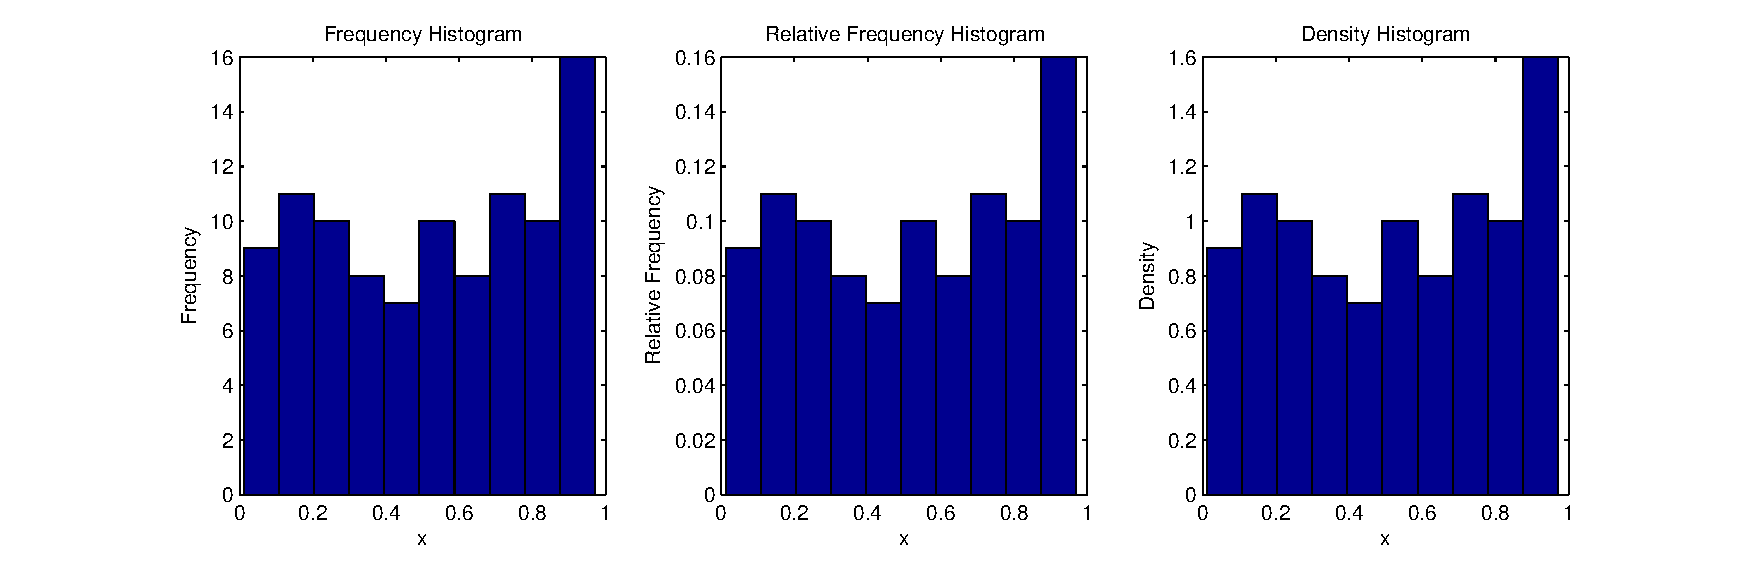
\includegraphics[width=6.5in]{figures/FreqRelFreqDensityHistograms100Unif01MT5489}}
\end{figure}

\begin{labwork}[Histograms with specified number of bins for univariate data]\label{LW:hist}
Let us use samples from the {\tt rand('twister',5489)} as our data set $x$ and plot various histograms.  Let us use {\tt hist} function (read {\tt help hist}) to make a default histogram with ten bins.  Then we can make three types of histogarms as shown in \hyperref[F:FreqRelFreqDensityHistograms100Unif01MT5489]{Figure~\ref*{F:FreqRelFreqDensityHistograms100Unif01MT5489}}  as follows:
\begin{VrbM}
>> rand('twister',5489);
>> x=rand(1,100); % generate 100 PRNs
>> hist(x) % see what default hist does in Figure Window
>> % Now let us look deeper into the last hist call
>> [Fs, Cs] = hist(x) % Cs is the bin centers and Fs is the frequencies of data set x
Fs =
     9    11    10     8     7    10     8    11    10    16
Cs =
    0.0598    0.1557    0.2516    0.3474    0.4433    0.5392    0.6351    0.7309    0.8268    0.9227
>> % produce a histogram plot the last argument 1 is the width value for immediately adjacent bars -- help bar
>> bar(Cs,Fs,1) % create a frequency histogram
>> bar(Cs,Fs/100,1) % create a relative frequency histogram
>> bar(Cs,Fs/(0.1*100),1) % create a density histogram (area of bars sum to 1)
>> sum(Fs/(0.1*100) .* ones(1,10)*0.1) % checking if area does sum to 1
>> ans = 1
\end{VrbM}
Try making a density histogram with 1000 samples from {\tt rand} with 15 bins.  You can specify the number of bins by adding an extra argument to {\tt hist}, for e.g. {\tt [Fs, Cs] = hist(x,15)} will produce 15 bins of equal width over the data range $\C{R}(x)$.
\end{labwork}

\begin{labwork}[Stem plots and ECDF plots for univariate data]\label{LW:StemEcdf}
We can also visualise the 100 data points in the array {\tt x} using stem plot and ECDF plot as shown in \hyperref[F:StemECDF100Unif01MT5489]{Figure~\ref*{F:StemECDF100Unif01MT5489}} as follows:
\begin{VrbM}
>> rand('twister',5489);
>> x=rand(1,100); % produce 100 samples with rand
>> stem(x,'.') % make a stem plot of the 100 data points in x (the option '.' gives solid circles for x)
>>% ECDF (type help ECDF) plot is extended to left and right by .2 and .6, respectively
>>% (second parameter 6 makes the dots in the plot smaller).
>> ECDF(x,6,.2,.6);
\end{VrbM}
\end{labwork}

\begin{figure}[htpb]
\caption{Frequency, Relative Frequency and Density Histograms\label{F:StemECDF100Unif01MT5489}}
\centering   \makebox{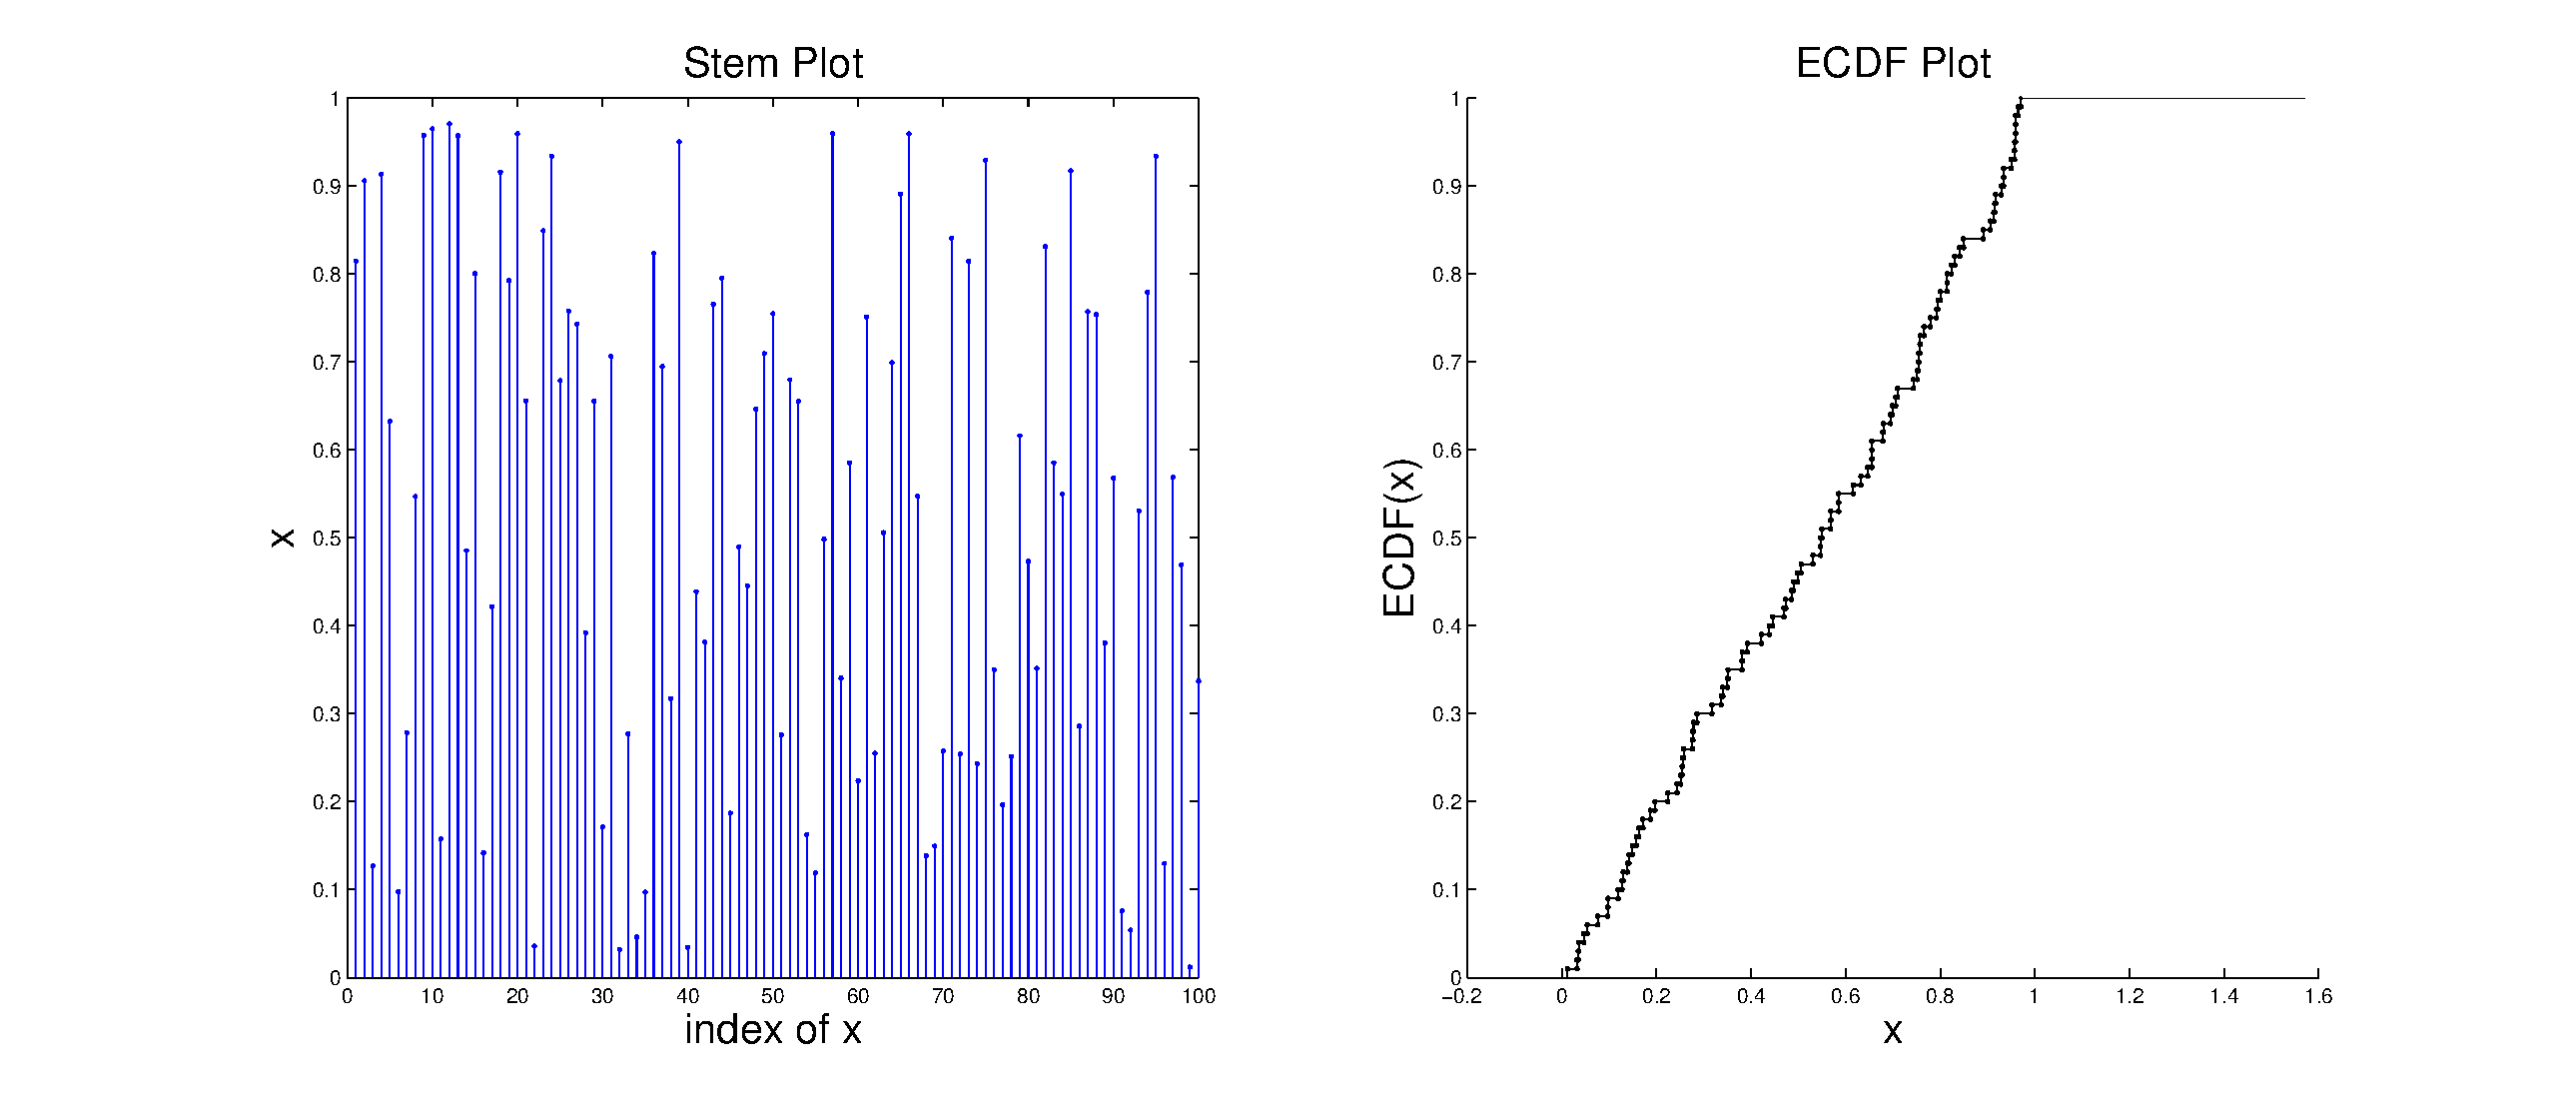
\includegraphics[width=6.5in]{figures/StemECDF100Unif01MT5489}}
\end{figure}

We can also visually summarise univariate data using the {\bf box plot} or {\bf box-whisker plot} available in the Stats Toolbox of {\sc Matlab}.  These family of plots display a set of sample quantiles, typically they are include, the median, the first and third quartiles and the minimum and maximum values of our data array $x$.

\subsection{Bivariate Data}
By bivariate data array $x$ we mean a $2 \times n$ matrix of real numbers or equivalently $n$ ordered pairs of points $(x_{1,i},x_{2,i})$ as $i=1,2,\ldots,n$.  The most elementary visualisation of these $n$ ordered pairs is in orthogonal Cartesian co-ordinates.  Such plots are termed 2D {\bf scatter plots} in statistics.
\begin{labwork}[Visualising bivariate data]\label{LW:2DScatter}
Let us generate a $2 \times 5$ array representing samples of $5$ ordered pairs sampled uniformly at random over the unit square $[0,1] \times [0,1]$.  We can make 2D scatter plot as shown in \hyperref[F:Twister5489X2x5Scatter2D]{Figure~\ref*{F:Twister5489X2x5Scatter2D}}  as follows:
\begin{VrbM}
>> rand('twister',5489);
>> x=rand(2,5)% create a sequence of 5 ordered pairs uniformly from unit square [0,1]X[0,1]
x =
    0.8147    0.1270    0.6324    0.2785    0.9575
    0.9058    0.9134    0.0975    0.5469    0.9649
>> plot(x(1,:),x(2,:),'x') % a 2D scatter plot with marker cross or 'x'
>> plot(x(1,:),x(2,:),'x', 'MarkerSize',15) % a 2D scatter plot with marker cross or 'x' and larger Marker size
>> xlabel('x_1'); ylabel('x_2'); % label the axes
\end{VrbM}
\end{labwork}

\begin{figure}[htpb]
\caption{2D Scatter Plot\label{F:Twister5489X2x5Scatter2D}}
\centering   \makebox{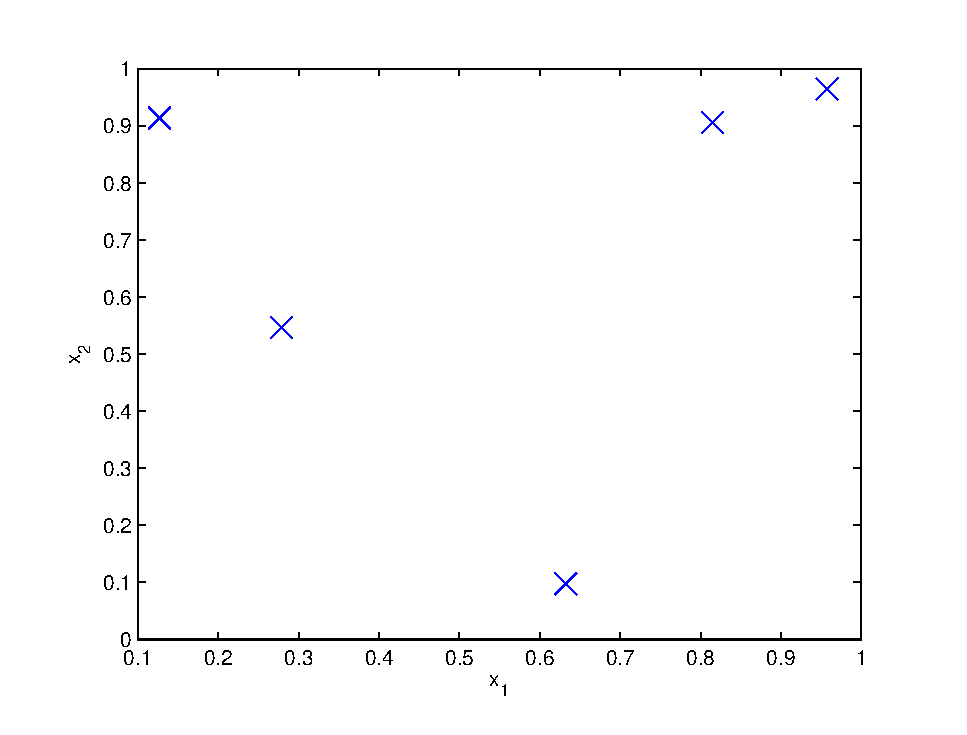
\includegraphics[width=4.5in]{figures/Twister5489X2x5Scatter2D}}
\end{figure}

There are several other techniques for visualising bivariate data, including,
2D histograms, surface plots, heat plots, and we will encounter some of them in the sequel.

\subsection{Trivariate Data}
Trivariate data is more difficult to visualise on paper but playing around with the rotate 3D feature in \Matlab's Figure window can help bring a lot more perspective.

\begin{labwork}[Visualising trivariate data]\label{LW:3DScatter}
We can make {\bf 3D scatter plots} as shown in \hyperref[F:Twister5489X3x5Scatter3D]{Figure~\ref*{F:Twister5489X3x5Scatter3D}}  as follows:
\begin{VrbM}
>> rand('twister',5489);
>> x=rand(3,5)% create a sequence of 5 ordered triples uniformly from unit cube [0,1]X[0,1]X[0,1]
x =
    0.8147    0.9134    0.2785    0.9649    0.9572
    0.9058    0.6324    0.5469    0.1576    0.4854
    0.1270    0.0975    0.9575    0.9706    0.8003
>> plot3(x(1,:),x(2,:),x(3,:),'x') % a simple 3D scatter plot with marker 'x'
>>% a more interesting one with options that control marker type, line-style, 
>>% colour in [Red Green Blue] values and marker size - read help plot3 for more options
>> plot3(x(1,:),x(2,:),x(3,:),'Marker','*','LineStyle','none','Color',[1 0 1],'MarkerSize',15) 
>> plot3(x(1,:),x(2,:),x(3,:),'m*','MarkerSize',15) % makes same  figure as before but shorter to write
>> box on % turn on the box and see the effect on the Figure
>> grid on % turn on the grid and see the effect on the Figure
>> xlabel('x_1'); ylabel('x_2'); zlabel('x_3'); % assign labels to x,y and z axes
\end{VrbM}
Repeat the visualisation below with a larger array, say {\tt x=rand(3,1000)}, and use the rotate 3D feature in the Figure window to visually explore the samples in the unit cube.  Do they seem to be uniformly distributed inside the unit cube?
\end{labwork}

\begin{figure}[htpb]
\caption{3D Scatter Plot\label{F:Twister5489X3x5Scatter3D}}
\centering   \makebox{\includegraphics[width=4.5in]{figures/Twister5489X3x5Scatter3D}}
\end{figure}


There are several other techniques for visualising trivariate data, including,
iso-surface plots, moving surface or heat plots, and you will encounter some of them in the future.

\subsection{Multivariate Data}
For high-dimensional data in $d$-dimensional space $\Rz^d$ with $d \geq 3$ you have to look at several lower dimensional projections of the data.  We can simultaneously look at 2D scatter plots for every pair of co-ordinates $\{(i,j) \in \{1,2,\ldots,d\}^2 : i \neq j \}$ and at histograms for every co-ordinate $i \in \{1,2,\ldots,d\}$ of the $n$ data points in $\Rz^d$.  Such a set of low-dimensional projections can be conveniently represented in a $d \times d$ matrix of plots called a {\bf matrix plot}. 

\begin{figure}[htpb]
\caption{Plot Matrix of uniformly generated data in $[0,1]^5$\label{F:Twister5489X100x5PlotMatrixFirst6andAll100}}
\centering
\mbox{\subfigure[First six samples]{\hspace{-1.cm} 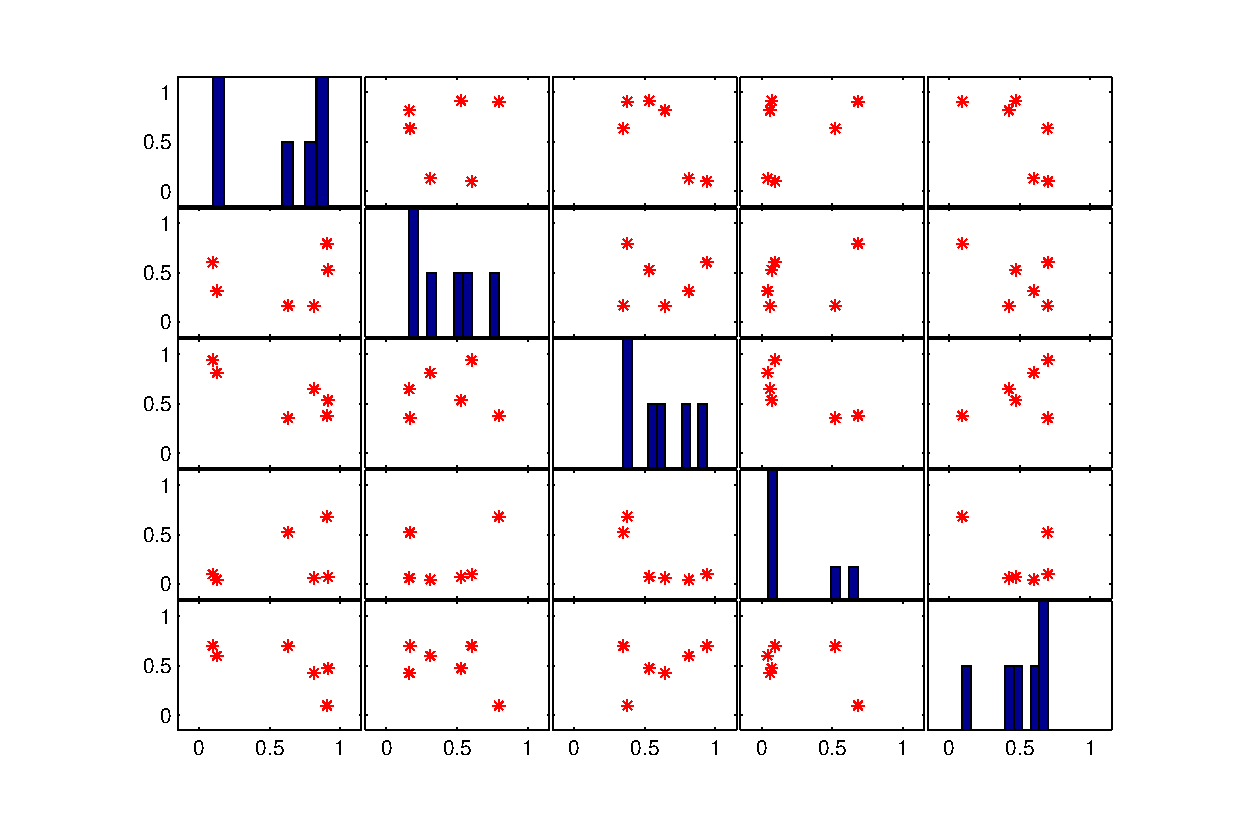
\includegraphics[width=3.750in]{figures/Twister5489X100x5PlotMatrixFirst6}} \hspace{-1.cm}
	   \subfigure[All thousand samples]{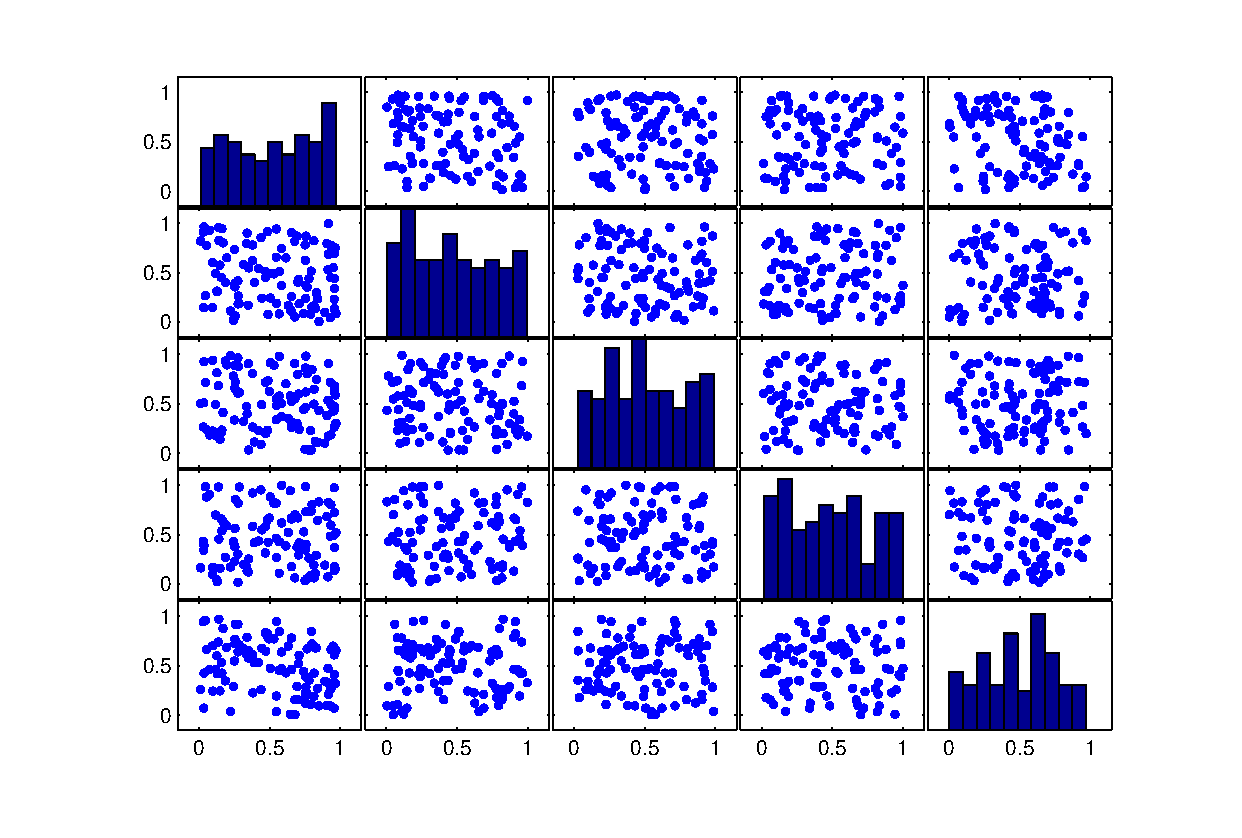
\includegraphics[width=3.750in]{figures/Twister5489X100x5PlotMatrixAll100}} }
\end{figure}

\begin{labwork}\label{LW:matrixplot5DUniform}
Let us make matrix plots from a uniformly generated  sequence of $100$ points in 5D unit cube $[0,1]^5$ as shown in \hyperref[F:Twister5489X100x5PlotMatrixFirst6andAll100]{Figure~\ref*{F:Twister5489X100x5PlotMatrixFirst6andAll100}}.
\begin{VrbM}
>> rand('twister',5489);
>> % generate a sequence of 1000 points uniformly distributed in 5D unit cube [0,1]X[0,1]X[0,1]X[0,1]X[0,1]
>> x=rand(1000,5);
>> x(1:6,:) % first six points in our 5D unit cube, i.e., the first six rows of x
ans =
    0.8147    0.6312    0.7449    0.3796    0.4271
    0.9058    0.3551    0.8923    0.3191    0.9554
    0.1270    0.9970    0.2426    0.9861    0.7242
    0.9134    0.2242    0.1296    0.7182    0.5809
    0.6324    0.6525    0.2251    0.4132    0.5403
    0.0975    0.6050    0.3500    0.0986    0.7054
>> plotmatrix(x(1:5,:),'r*') % make a plot matrix
>> plotmatrix(x) % make a plot matrix of all 1000 points
\end{VrbM}
\end{labwork}


\section{Loading and Exploring Real-world Data}\label{S:EDA}

All of the data we have played with so far were computer-generated.  It is time to get our hands dirty with real-world data.  The first step is to obtain the data.  
Often, publicly-funded institutions allow the public to access their databases.  Such data can be fetched from appropriate URLs in one of the two following ways: 
\begin{itemize}
\item[{\sf Method~A}:] Manually download by filling the appropriate fields in an online request form.
\item[{\sf Method~B}:] Automagically download directly from your \Matlab session.
\end{itemize}
Then we want to inspect it for inconsistencies, missing values and replace them with {\tt NaN} values in \Matlab that stand for not-any-number.  Finally, we can visually explore, transform and interact with the data to discover interesting patterns that are hidden in the data.  This process is called {\em exploratory data analysis} and is the foundational first step towards subsequent computational statistical experiments [{\em John W.~Tukey, Exploratory Data Analysis, Addison-Wesely, New York, 1977}].

\subsection{Geological Data}
 Let us focus on the data of earth quakes that heavily damaged Christchurch on February 22 2011.  This data can be fetched from the URL \href{http://magma.geonet.org.nz/resources/quakesearch/}{\url{http://magma.geonet.org.nz/resources/quakesearch/}} by {\sf Method A} and loaded into \Matlab for exploratory data analysis as done in \hyperref[LW:NZEQChCch20110222]{Labwork~\ref*{LW:NZEQChCch20110222}}.
 
 \begin{labwork}\label{LW:NZEQChCch20110222}
Let us go through the process one step at a time using {\sf Method~A}.  
\begin{enumerate}
\item Download the data as a CSV or {\em comma separated variable} file in plain ASCII text (this has been done for this data already for you and saved as {\tt NZ20110222earthquakes.csv} in the {\tt CSEMatlabScripts} directory).
\item Open the file in a simple text editor such as {\tt Note Pad} in Windows or one of the following editors in OS X, Unix, Solaris, Linux/GNU variants such as Ubuntu, SUSE, etc: {\tt vi}, {\tt vim}, {\tt emacs}, {\tt geany}, etc.  The first three and last two lines of this file look as follows:
\begin{VrbM} 
CUSP_ID,LAT,LONG,NZMGE,NZMGN,ORI_YEAR,ORI_MONTH,ORI_DAY,ORI_HOUR,ORI_MINUTE,ORI_SECOND,MAG,DEPTH
3481751,-43.55432,172.68898,2484890,5739375,2011,2,22,0,0,31.27814,3.79,5.8559,
3481760,-43.56579,172.70621,2486287,5738106,2011,2,22,0,0,43.70276,3.76,5.4045,
.
.
.
3469114,-43.58007,172.67126,2483470,5736509,2011,2,22,23,28,11.1014,3.117,3,
3469122,-43.55949,172.70396,2486103,5738805,2011,2,22,23,50,1.06171,3.136,12,
\end{VrbM}
The thirteen columns correspond to fairly self-descriptive features of each measured earth quake given in the first line or row.  They will become clear in the sequel.  Note that the comma character (`{\tt ,}') separates each unit or measurement or descpiption in any CSV file.

\item The next set of commands show you how to load,  manipulate and visually explore this data.

\begin{VrbM}
%% Load the data from the comma delimited text file 'NZ20110222earthquakes.csv' with 
%% the following column IDs
%% CUSP_ID,LAT,LONG,NZMGE,NZMGN,ORI_YEAR,ORI_MONTH,ORI_DAY,ORI_HOUR,ORI_MINUTE,ORI_SECOND,MAG,DEPTH
%% Using MATLAB's dlmread command we can assign the data as a matrix to EQ; 
%% note that the option 1,0 to dlmread skips first row of column descriptors
%
% the variable EQall is about to be assigned the data as a matrix
EQall = dlmread('NZ20110222earthquakes.csv', ',' , 1, 0); 
size(EQall) % report the dimensions or size of the matrix EQall
ans =
   145    14
\end{VrbM}

\item In order to understand the syntax in detail get {\tt help} from \Matlab!
\begin{VrbM}
>> help dlmread
 DLMREAD Read ASCII delimited file.
 .
 .
 .
 \end{VrbM}
 
\item When there are units in the CSV file that can't be converted to floating-point numbers, it is customary to load them as a {\tt NaN} or {\em Not-a-Number} value in \Matlab.  So, let's check if there are any rows with {\tt NaN} values and remove them from our analysis.  Note that this is not the only way to deal with missing data! After that let's remove any locations outside Christchurch and its suburbs (we can find the latitude and longitude bounds from online resources easily) and finally view the 4-tuples of (latitude, longitude, magnitude, depth) for each measured earth quake in Christchurch on February 22 of 2011 as a scatter plot shown in \hyperref[F:NZEQ20110222ChchLtLnMgDpScatterMatrixPlot]{Figure~\ref*{F:NZEQ20110222ChchLtLnMgDpScatterMatrixPlot}} (the axes labels were subsequently added from clicking {\tt <Edit>} and {\tt <Figure Properties...>} tabs of the output Figure Window).
 \begin{VrbM}
>> EQall(any(isnan(EQall),2),:) = []; %Remove any rows containing NaNs from the matrix EQall
>> % report the size of EQall and see if it is different from before we removed and NaN containing rows
>> size(EQall) 
ans =   145    14
>> % remove locations outside Chch and assign it to a new variable called EQ
>> EQ = EQall(-43.75<EQall(:,2) & EQall(:,2)<-43.45 ... 
              & 172.45<EQall(:,3) & EQall(:,3)<172.9 & EQall(:,12)>3, :);
>> % now report the size of the earthquakes in Christchurch in variable EQ
>> size(EQ)
ans =   124    14
>> % assign the four variables of interest
>> LatData=EQ(:,2); LonData=EQ(:,3); MagData=EQ(:,12); DepData=EQ(:,13);
>> % finally make a plot matrix of these 124 4-tuples as red points 
>> plotmatrix([LatData,LonData,MagData,DepData], 'r.');
\end{VrbM}
\end{enumerate}
All of these commands have been put in a script M-file {\tt NZEQChCch20110222.m} in \hyperref[Mf:NZEQChCch20110222]{Labwork~\ref*{Mf:NZEQChCch20110222}} and you can simply call it from the command window to automatically load the data and assign it to the variables {\tt EQAll} {\tt EQ}, {\tt LatData}, {\tt LonData}, {\tt MagData} and {\tt DepData}, instead of retyping each command above every time you need these matrices in \Matlab, as follows:
\begin{VrbM}
>> NZEQChCch20110222
ans =   145    14
ans =   145    14
ans =   124    14
\end{VrbM}
In fact, we will do exactly this to conduct more exploratory data analysis with these earth quake measurements in \hyperref[LW:NZEQChCch20110222EDA]{Labwork~\ref*{LW:NZEQChCch20110222EDA}}.
\end{labwork}

\begin{figure}[htpb]
\caption{Matrix of Scatter Plots of the latitude, longitude, magnitude and depth of the 22-02-2011 earth quakes in Christchurch, New Zealand.\label{F:NZEQ20110222ChchLtLnMgDpScatterMatrixPlot}}
\centering   \makebox{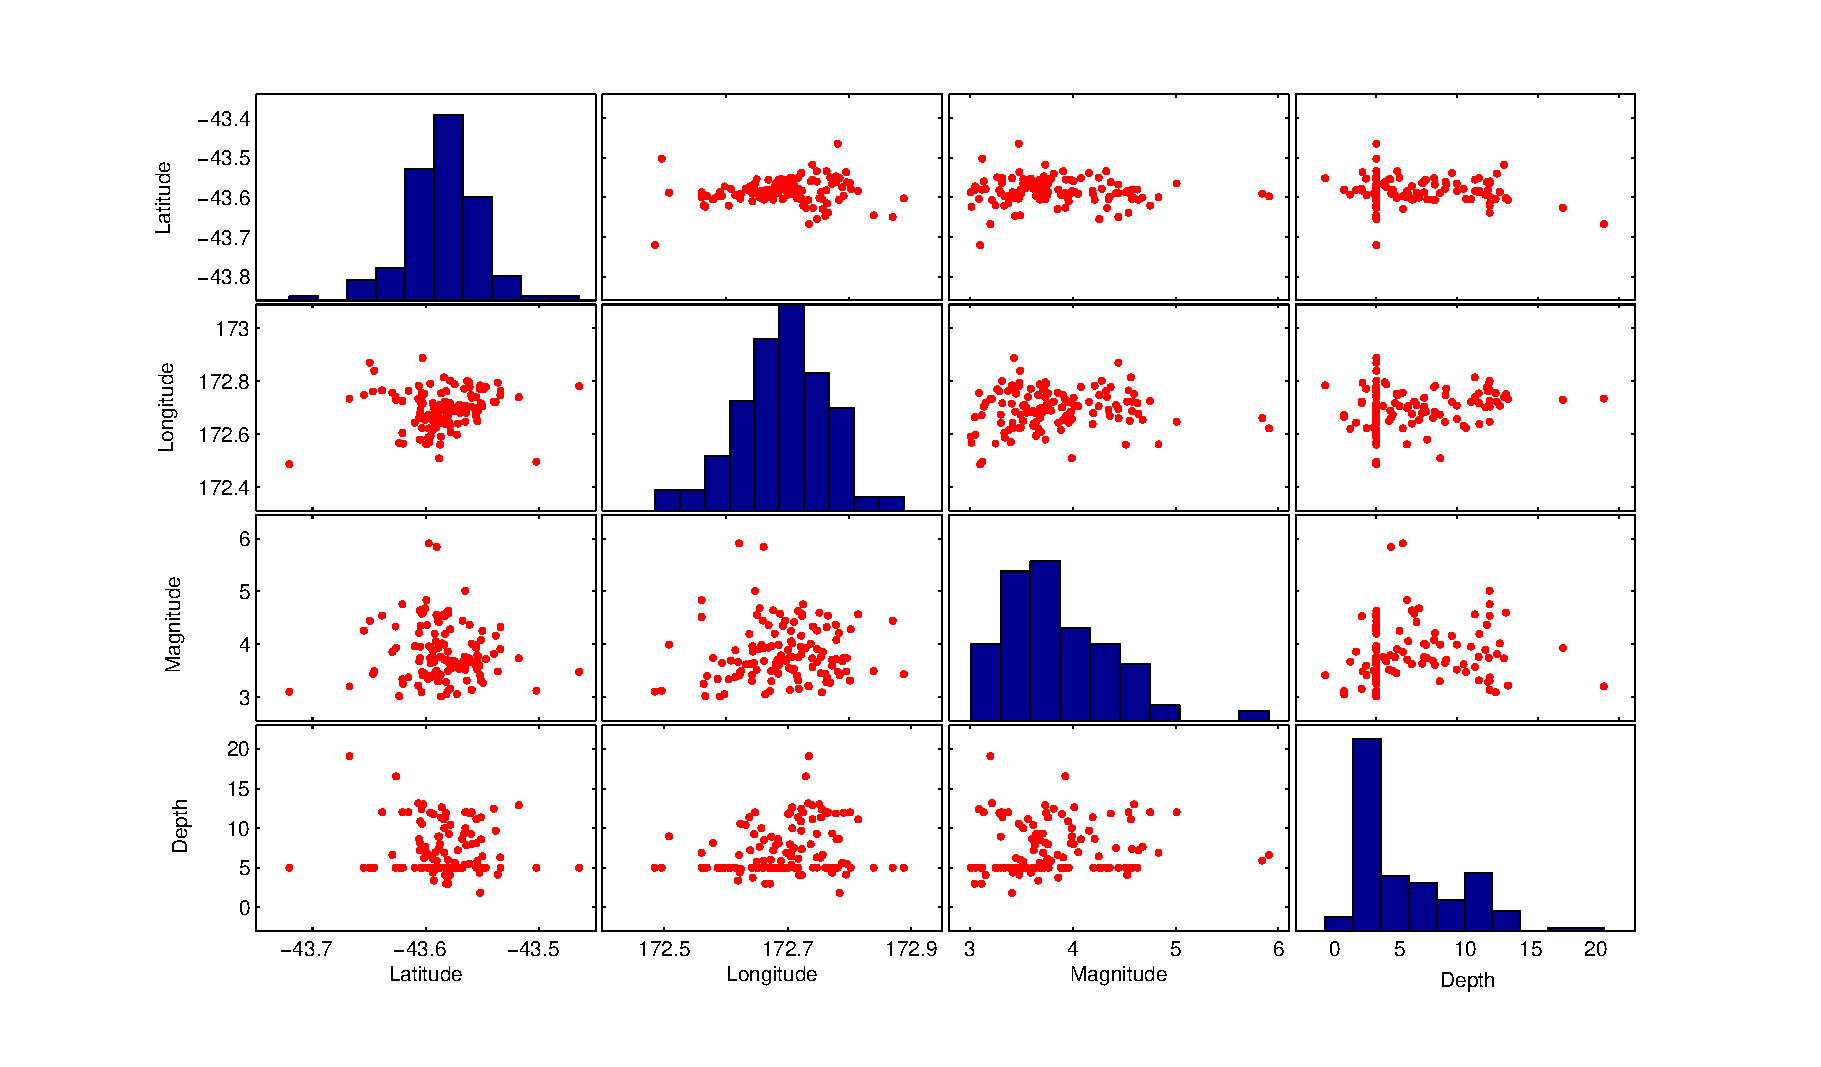
\includegraphics[width=6.5in]{figures/NZEQ20110222ChchLtLnMgDpScatterMatrixPlot}}
\end{figure}


\begin{labwork}\label{LW:NZEQChCch20110222EDA}
Try to understand how to manipulate time stamps of events in \Matlab and the Figures being output by following the comments in the script file {\tt NZEQChCch20110222EDA.m}.
\begin{VrbM}
>> NZEQChCch20110222
ans =   145    14
ans =   145    14
ans =   124    14
ans =   145    14
ans =   145    14
ans =   124    14
ans = 22-Feb-2011 00:00:31
ans = 22-Feb-2011 23:50:01
\end{VrbM}
\VrbMf[label=NZEQChCch20110222EDA.m]{scripts/NZEQChCch20110222EDA.m}
\end{labwork}

\subsubsection{Geostatistical exploratory data analysis with Google Earth}

\begin{figure}[htpb]
\caption{Google Earth Visualisation of the earth quakes\label{F:NZEQ20110222ChchLtLnMgDpInGoogleEarthViewFromUSGS}}
\centering   \makebox{\includegraphics[width=4.5in]{figures/NZEQ20110222ChchLtLnMgDpInGoogleEarthViewFromUSGS}}
\end{figure}

A global search at \href{http://neic.usgs.gov/cgi-bin/epic/epic.cgi}{\url{http://neic.usgs.gov/cgi-bin/epic/epic.cgi}}
%%?SEARCHMETHOD=1&FILEFORMAT=7&SEARCHRANGE=PP&SYEAR=2011&SMONTH=2&SDAY=22&EYEAR=2011&EMONTH=2&EDAY=22&LMAG=&UMAG=&NDEP1=&NDEP2=&IO1=&IO2=&CLAT=0.0&CLON=0.0&CRAD=0.0&SUBMIT=Submit+Search}
with the following parameters:
\begin{verbatim}
Date Range: 2011 2 22 to 2011 2 22 
Catalog: USGS/NEIC (PDE-Q) 
\end{verbatim}
produced 43 earth quakes world-wide, including those in Christchurch as shown in \hyperref[F:NZEQ20110222ChchLtLnMgDpInGoogleEarthViewFromUSGS]{Figure~\ref*{F:NZEQ20110222ChchLtLnMgDpInGoogleEarthViewFromUSGS}}.  One can do a lot more than a mere visualisation with the USGS/NEIC  database of earth-quakes wolrd-wide, the freely available {\tt Google earth} software bundle \href{http://www.google.com/earth/index.html}{\url{http://www.google.com/earth/index.html}} and the freely available \Matlab package {\tt googleearth} from \href{http://www.mathworks.com/matlabcentral/fx_files/12954/4/content/googleearth/html/html_product_page.html}{\url{http://www.mathworks.com/matlabcentral/fx_files/12954/4/content/googleearth/html/html_product_page.html}}.

\subsection{Metereological Data}

New Zealand's meteorological service NIWA provides weather data under it TERMS AND CONDITIONS FOR ACCESS TO DATA (See \url{http://cliflo.niwa.co.nz/doc/terms_print.html}).  We will explore some data of rainfall and temperatures from NIWA.

\subsubsection{Daily Rainfalls in Christchurch}

%Rainfall Data in Christchurch

Automagic downloading of the data by {\sf Method B} can be done if the data provider allows automated queries.  It can be accomplished by {\tt urlread} for instance.  %Try to download the file



%is being  \work.  But you can t

Paul Brouwers has a basic CliFlo datafeed on \url{http://www.math.canterbury.ac.nz/php/lib/cliflo/rainfall.php}.  %?range=20100425:20100501
This returns the date and rainfall in milli meters as measured from the CHCH aeroclub station. It is assumed that days without readings would not be listed. %It expects a range parameter such as: ?range=20100425:20100501 The first number is the starting search date (YYYYMMDD). Colon as separator. The first number is the ending search date (YYYYMMDD). CliFlo limits us to 2 million rows for the subscription and 40,000 rows per query (which is equivalent of over 100 years of data, so I we're safe - 
The data doesn't go back much before 1944.

%wetdataURL = 'http://www.math.canterbury.ac.nz/php/lib/cliflo/?range=20100101:20100510' wetdataURL = 'http://www.math.canterbury.ac.nz/php/lib/cliflo/rainfall.php'
%\work 


\begin{labwork}\label{LW:ChchDailyRainfallSince}
Understand how \hyperref[F:ChchDailyRainfallSince]{Figure~\ref*{F:ChchDailyRainfallSince}} is obtained by the script file {\tt RainFallsInChch.m} by typing and following the comments:

\begin{VrbM}
>> RainFallsInChch
RainFallsChch =     [24312x1 int32]    [24312x1 double]
ans =       24312           2
FirstDayOfData =    19430802
LastDayOfData =    20100721
\end{VrbM}

\VrbMf[label=RainFallsInChch.m]{scripts/RainFallsInChch.m}
\end{labwork}

\begin{figure}[htpb]
\caption{Daily rainfalls in Christchurch since March 27 2010 \label{F:ChchDailyRainfallSince}}
\centering   \makebox{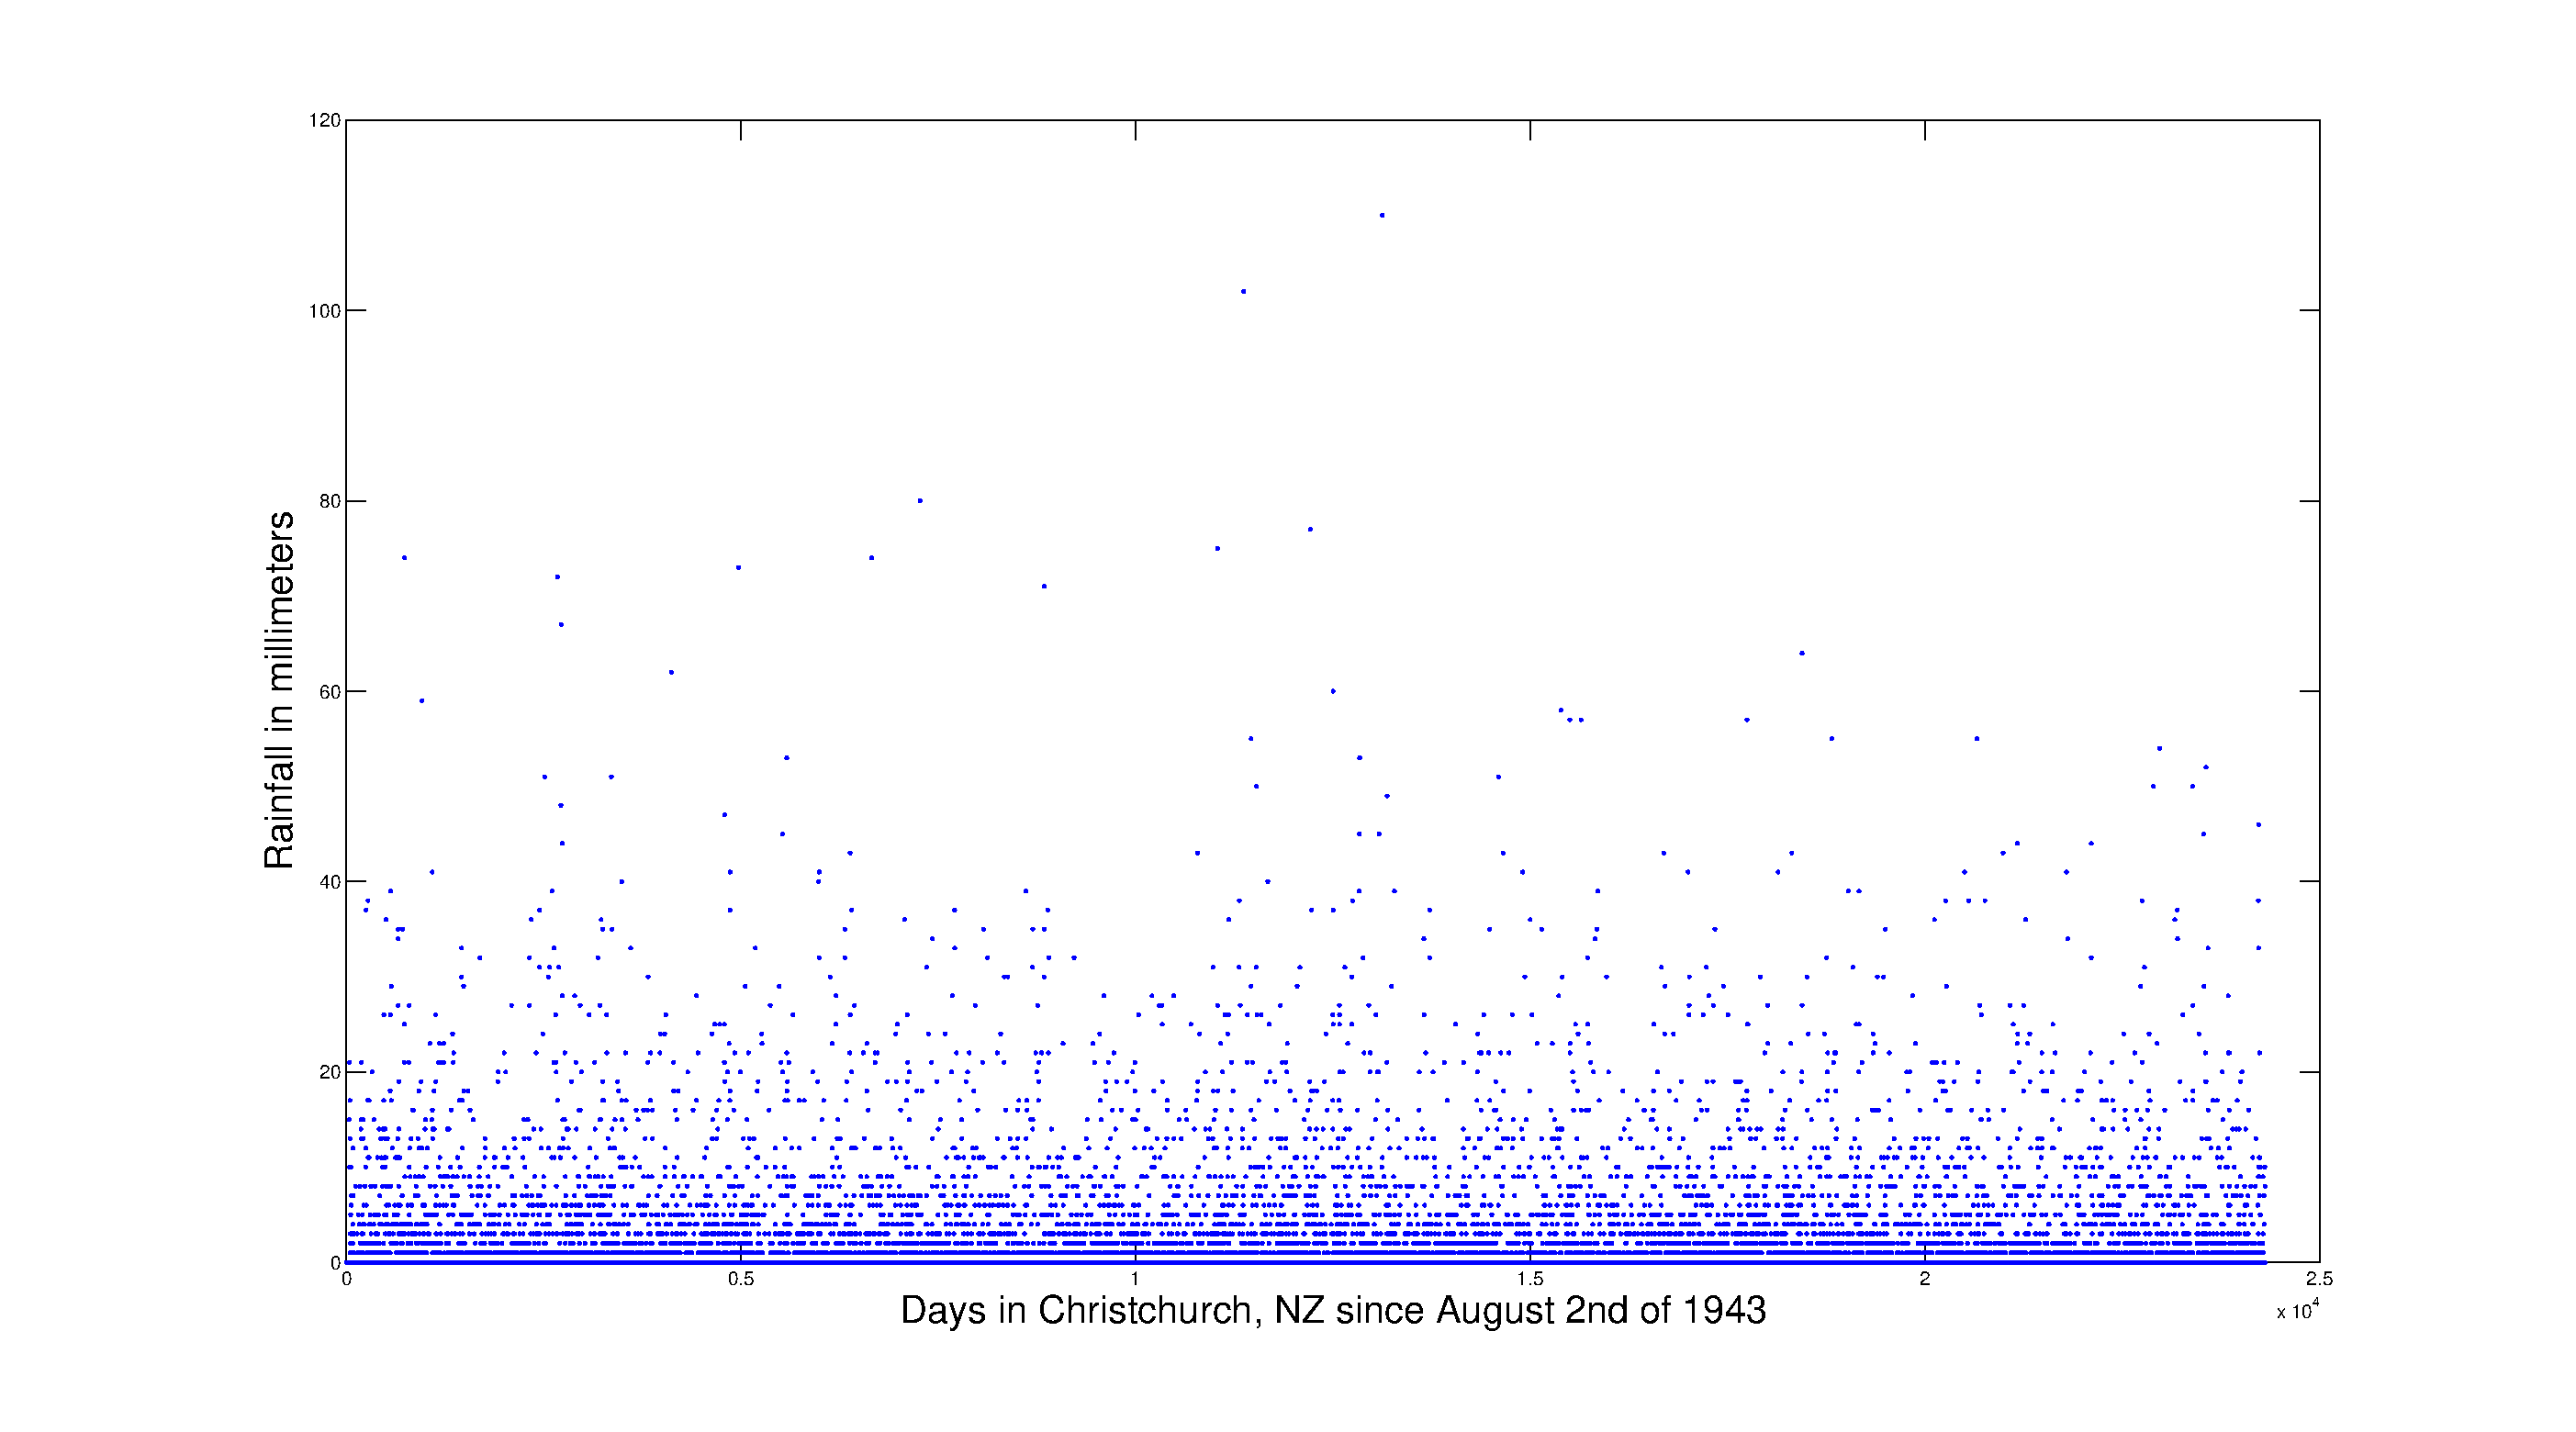
\includegraphics[width=6.5in]{figures/ChchDailyRainfallSince}}
\end{figure}

\subsubsection{Daily Temperatures in Christchurch}


\begin{labwork}\label{LW:ChchTempsLoad}
Understand how \hyperref[F:ChchTemps365DaysSince20100327]{Figure~\ref*{F:ChchTemps365DaysSince20100327}} is being generated by following the comments in the script file {\tt ChchTempsLoad.m} by typing:
\begin{VrbM}
>> ChchTempsLoad
\end{VrbM}
\VrbMf[label=ChchTempsLoad.m]{scripts/ChchTempsLoad.m}
\end{labwork}

\begin{figure}[htpb]
\caption{Daily temperatures in Christchurch for one year since March 27 2010 \label{F:ChchTemps365DaysSince20100327}}
\centering   \makebox{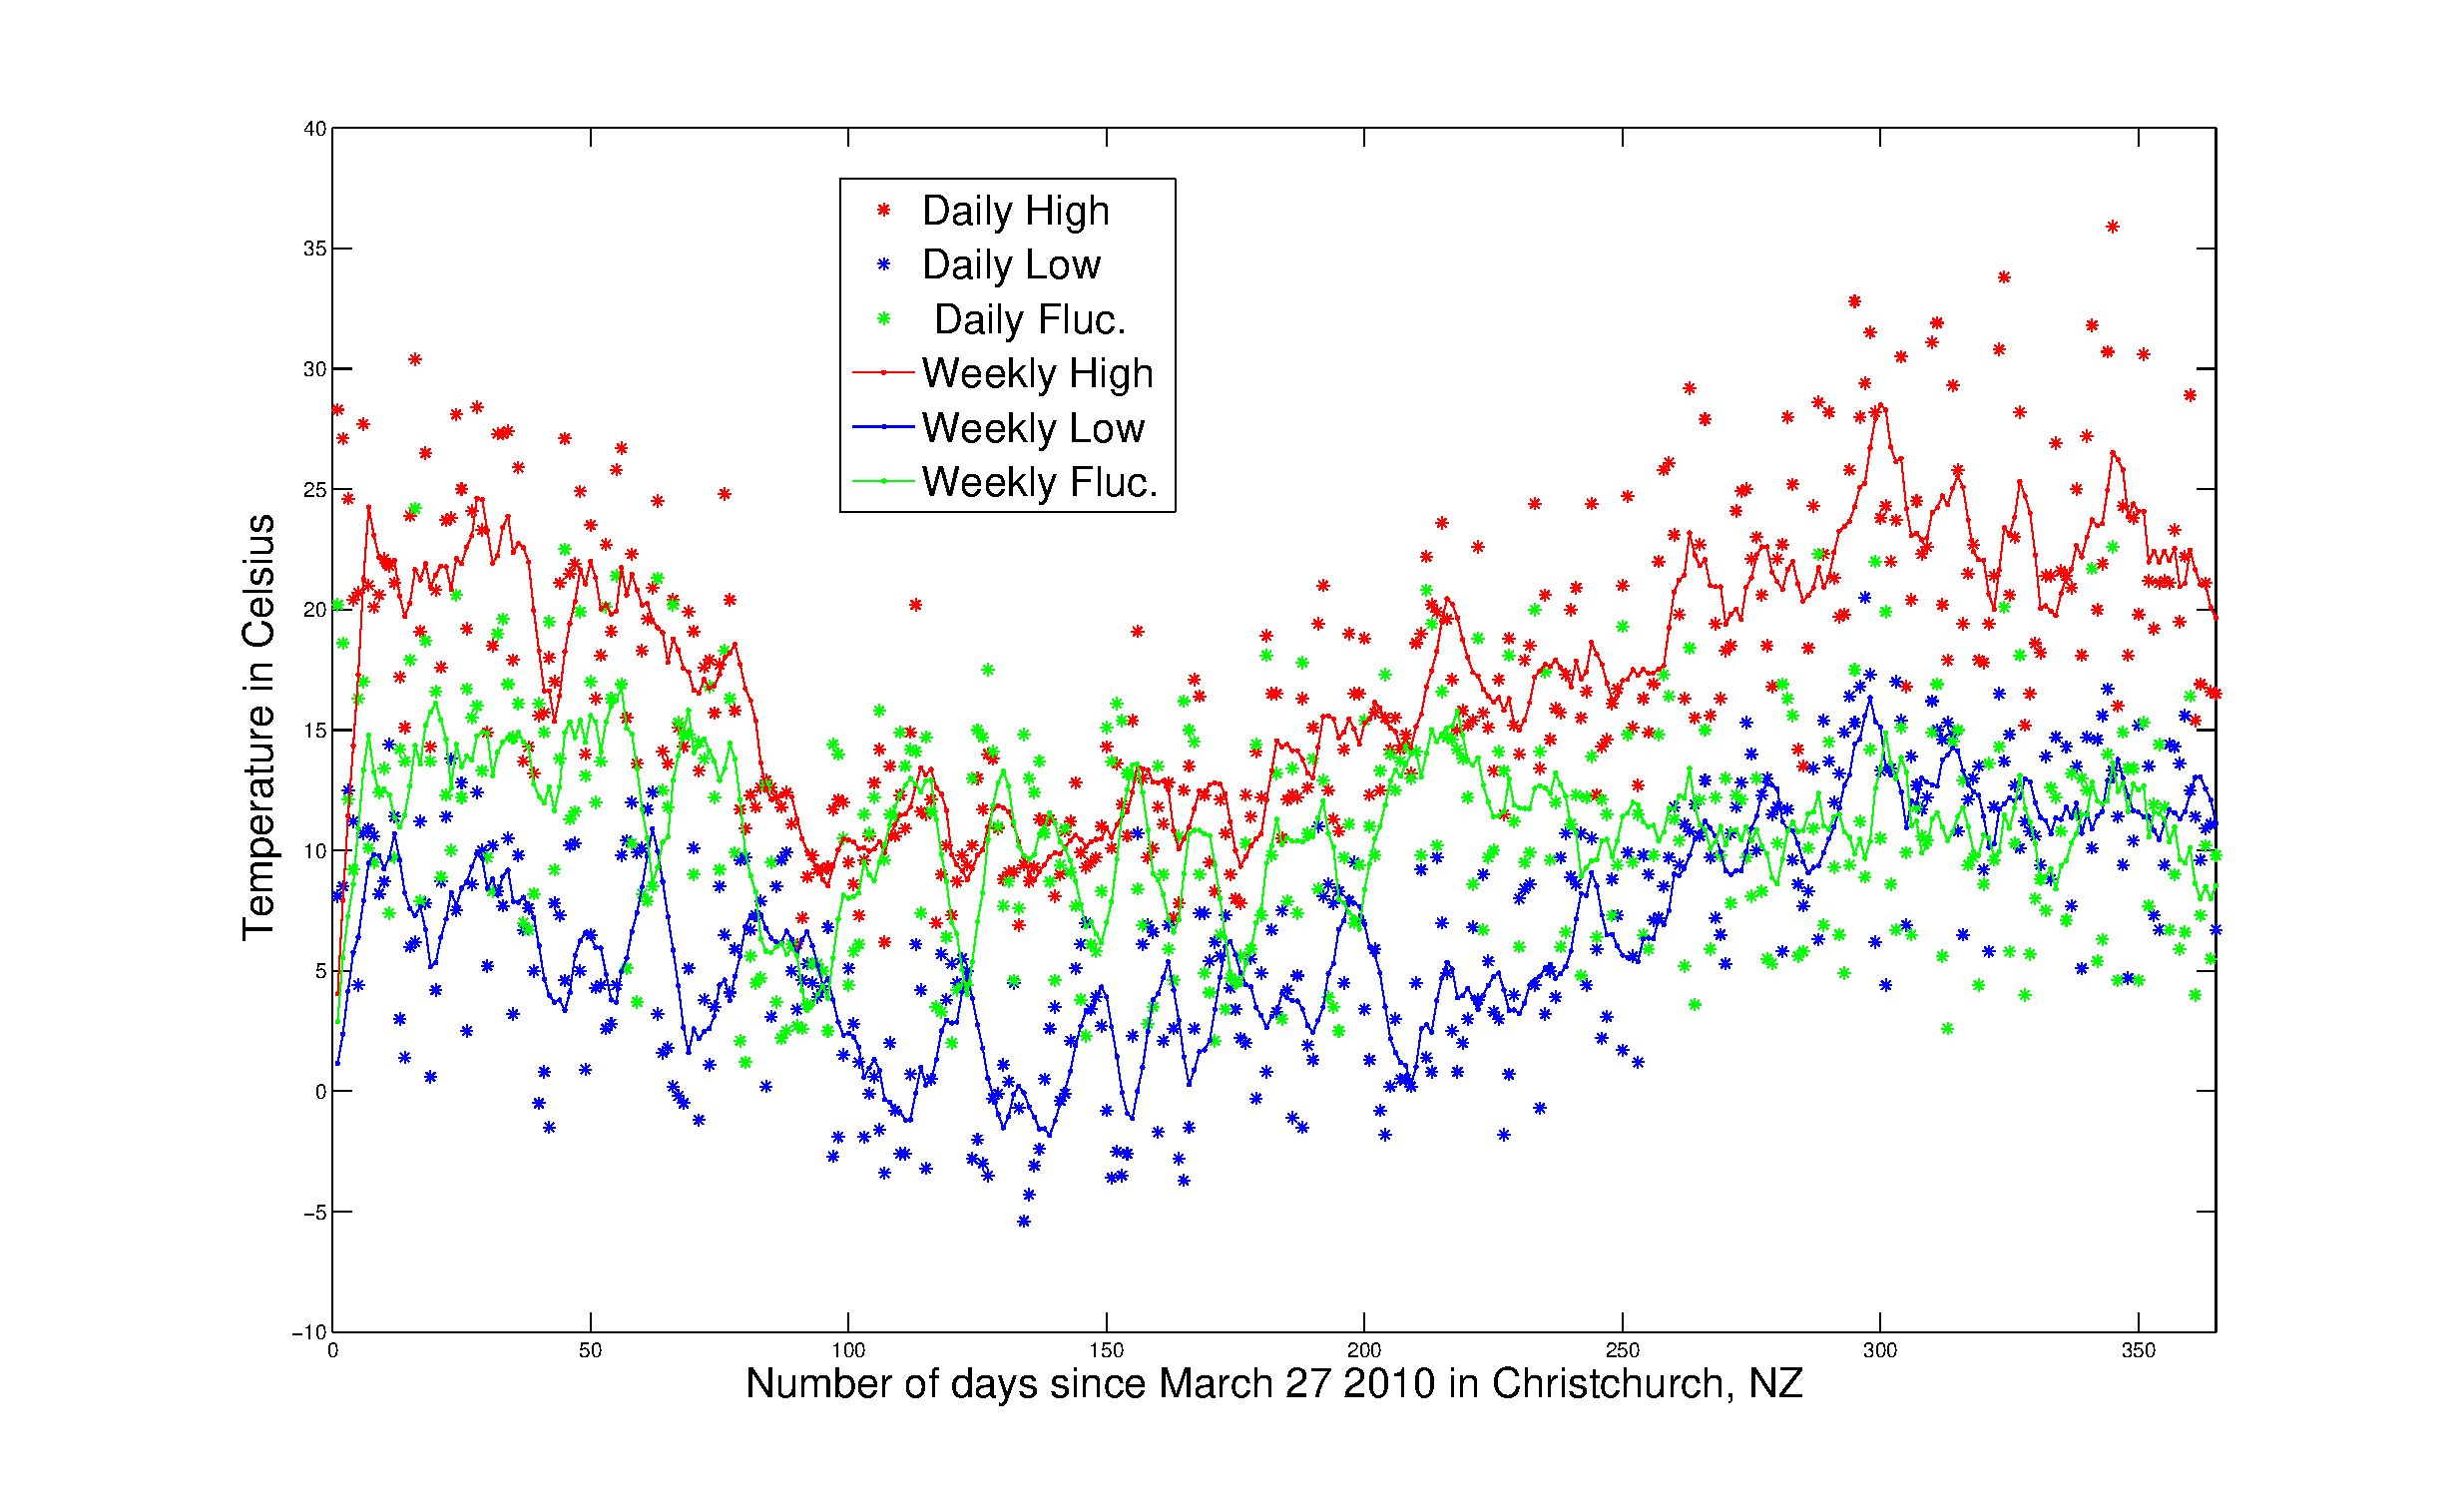
\includegraphics[width=6.5in]{figures/ChchTemps365DaysSince20100327}}
\end{figure}

\subsection{Textual Data}

Processing and analysing textual data to make a decision is another important computational statistical experiment. An obvious example  is machine translation and a less obvious one is exploratory data analysis of the textual content of 
\begin{itemize}
\item a large document
\item twitter messages within an online social network of interest
\item etc.
\end{itemize}

An interesting document with a current affairs projection is the Joint Operating Environment 2010 Report by the US Department of Defense.  This document was downloaded from \href{http://www.jfcom.mil/newslink/storyarchive/2010/JOE_2010_o.pdf}{\url{http://www.jfcom.mil/newslink/storyarchive/2010/JOE_2010_o.pdf}}.  The first paragraph of this 74 page document (JOE 2010 Reprort) reads:

{\small
ABOUT THIS STUDY The Joint Operating Environment is intended to inform joint concept development and experimentation throughout the Department of Defense. It provides a perspective on future trends, shocks, contexts, and implications for future joint force commanders and other leaders and professionals in the national security field. This document is speculative in nature and does not suppose to predict what will happen in the next twenty-five years. Rather, it is intended to serve as a starting point for discussions about the future security environment at the operational level of war. Inquiries about the Joint Operating Environment should be directed to USJFCOM Public Affairs, 1562 Mitscher Avenue, Suite 200, Norfolk, VA 23551-2488, (757) 836-6555. 

Distribution Statement A: Approved for Public Release
}

\begin{figure}[htpb]
\caption{Wordle of JOE 2010\label{F:joe_vs_wordle}}
\centering   \makebox{\includegraphics[width=6.5in]{figures/joe_vs_wordle_RaazCroppedPhilWilsonsImage}}
\end{figure}

We can try to produce a statistic of this document by recording the frequency of words in its textual content. Then we can produce a ``word histogram'' or ``word cloud'' to explore the document visually at one of the coarsest possible resolutions of the textual content in the JOE 2010 Report.  The ``word cloud'' shown in \hyperref[F:joe_vs_wordle]{Figure~\ref*{F:joe_vs_wordle}} was produced by Phillip Wilson using {\em wordle} from \href{http://www.wordle.net/}{\url{http://www.wordle.net/}}.  A description from the wordle URL says:

{\small
Wordle is a toy for generating �word clouds� from text that you provide. The clouds give greater prominence to words that appear more frequently in the source text. You can tweak your clouds with different fonts, layouts, and color schemes. The images you create with Wordle are yours to use however you like. You can print them out, or save them to the Wordle gallery to share with your friends.
}

\begin{labwork}[favourite word cloud]\label{LW:JoeWordle}  This is just for fun.  Produce a ``word cloud'' of your honours thesis or summer project or any other document that fancies your interest by using {\em wordle} from \href{http://www.wordle.net/}{\url{http://www.wordle.net/}}. Play with the aesthetic features to change colour, shapes, etc.\end{labwork}

\subsection{Machine Sensor Data}

Instrumentation of modern machines, such as planes, rockets and cars allow the sensors in the machines to collect live data and dynamically take {\em decisions} and subsequent {\em actions} by executing algorithms to drive their devices in response to the data that is streaming into their sensors.  For example, a rocket may have to adjust its boosters to compensate for the prevailing directional changes in wind in order to keep going up and launch a satellite.  
These types of decisions and actions, theorised by {\em controlled Markov processes}, typically arise in various fields of engineering such as, aerospace, civil, electrical, mechanical, robotics, etc.

In an observational setting, without an associated control problem, one can use machine sensor data to get information about some state of the system or phenomenon, i.e., what is it doing? or where is it?, etc.  Sometimes sensors are attached to a sample of individuals from a  wild population, say Emperor Penguins in Antarctica where the phenomenon of interest may be the diving habits of this species after the eggs hatch.  As an other example we can attach sensors to a double pendulum and find what it is doing when we give it a spin.

Based on such observational data the experimenter typically tries to learn about the behaviour of the system from the sensor data to estimate parameters, test hypotheses, etc. Such types of experiments are typically performed by scientists in various fields of science, such as, astronomy, biology, chemistry, geology, physics, etc.  

\subsubsection{Chaotic Time Series of a Double Pendulum}

\begin{figure}[htbp]
\begin{center}
{\scriptsize
\begin{tabular}{ccc}
A: DP Schematic & B: Streaming DP data & C: Enclosures of two initially close trajectories\\
  \includegraphics[scale=0.5]{figures/dp} &
  \includegraphics[scale=0.66]{figures/vlcsnap-2010-01-13-10h11m08s38_closeup} &
  \includegraphics[height=3cm,width=6.75cm]{figures/divergence_piers}
\end{tabular}
}
\end{center}
\caption{Double Pendulum}
\label{F:DP3}
\end{figure}

Sensors called {\em optical encoders} have been attached to the top end of each arm of a chaotic double pendulum in order to obtain the angular position of each arm through time as shown in \hyperref[F:DP3]{Figure~\ref*{F:DP3}}.  Time series of the angular position of each arm for two trajectories that were initialized very similarly, say the angles of each arm of the double pendulum are almost the same at the initial time of release.  Note how quickly the two trajectories diverge!  System with such a sensitivity to initial conditions are said to be {\em chaotic}.

\begin{labwork}[A Challenging Task]\label{LW:DPtrajectoryparsing}  Try this if you are interested.  Read any of the needed details about the design and fabrication of  the double pendulum at \href{http://www.math.canterbury.ac.nz/~r.sainudiin/lmse/double-pendulum/}{\url{http://www.math.canterbury.ac.nz/~r.sainudiin/lmse/double-pendulum/}}.  Then use \Matlab to generate a plot similar to \hyperref[F:DP3]{Figure~\ref*{F:DP3}(C)} using time series data of {\sf trajectory~1} and {\sf  trajectory~2} linked from the bottom of the above URL.
 \end{labwork}

\comment{
\subsection{Biological Data}
\work
}
